\chapter{Математическая модель БОЭП как объекта управления} \label{ch:ch3}

Оптико-электронный прибор (ОЭП) вертолетного базирования имеет тепловизионный и телевизионный каналы, лазерный дальномер. Кроме того, на борту устанавливают оптико-электронную систему постановки помех (СОЭП). Управление направлением линии визирования осуществляется перемещением всего оптико-электронного блока. Для ОЭП и СОЭП конструктивно оптико-электронный блок представляет собой блок, в котором размещены оптические приборы, вращающийся по углу места внутри вилки, вращающейся по углу азимута 
(рисунок~\ref{fig:device}, кинематическая схема на рисунке~\ref{fig:kinematic}). 
На осях вращения размещены моментные двигатели и датчики углов. ОЭП установлен в носовой части вертолета, СОЭП устанавливается в хвостовой части и на балках 
(рисунок~\ref{fig:helicopter}).

При проектировании ОЭП и СОЭП возникли задачи построения адекватной математической модели, синтеза системы управления направлением линии визирования и построения компьютерной имитационной модели ОЭП и СОЭП. Решение этих задач является продолжением работ [3/15-18]. Математическая модель строится на основе применения уравнений Лагранжа II-го рода с использованием смешанного метода Жильбера. 

\begin{comment}
Разработаны алгоритмы управления, обеспечивающие требуемые точностные и динамические характеристики СОЭП для режима слежения и наведения. Исследование динамических свойств СОЭП проводится с использованием компьютерной имитационной модели. Использование метода математического моделирования при проектировании бортовых СОЭП позволяет обеспечить достижение заложенных технических требований по параметрам системы, сократить сроки разработки, настройки и испытаний изделия. Компьютерная имитационная модель верифицирована по результатам настройки опытного образца.
\end{comment}

\begin{landscape}
\section{Принципиальная схема} \label{ch:ch3/sect1}

\begin{figure}[ht]
	\centering
	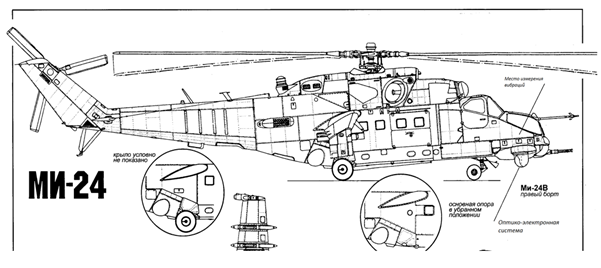
\includegraphics[width=1.0\linewidth]{img-15} 
	\caption{Принципиальная схема расположения на борту}
	\label{fig:helicopter}
\end{figure}

\begin{figure}[ht]
	\centering
	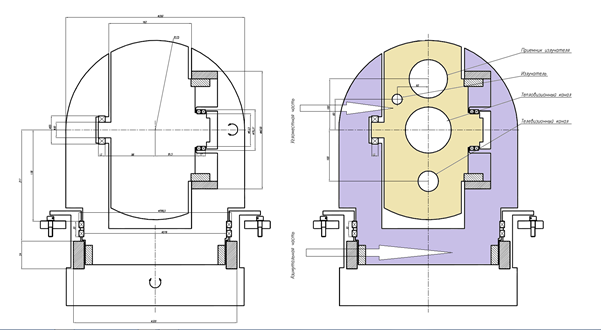
\includegraphics[width=1.0\linewidth]{img-16} 
	\caption{Общий вид изделия}
	\label{fig:device}
\end{figure}
\end{landscape}

\section{Механическая модель} \label{ch:ch3/sect2}

Исходя из анализа конструкции ОЭП для управления линией визирования оптико-электронного блока – объекта управления (ОУ) и движения вертолета (ЛА), на котором он установлен, приняты основные допущения, выбраны системы координат и определены исходные данные, необходимые для построения математической модели. ОУ.

\begin{figure}[ht]
	\centering
	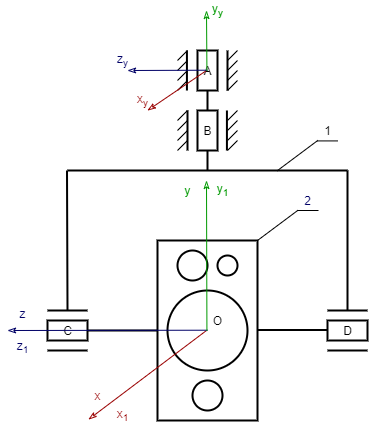
\includegraphics[width=0.5\linewidth]{cinematics} 
	\caption{Кинематическая схема}
	\label{fig:kinematic}
\end{figure}

\subsection{Основные допущения, системы координат} \label{sec:ch3/sec3}

\begin{enumerate}
	\item ОУ моделируется двумя абсолютно твердыми телами:
	\begin{itemize}
		\item 1–е тело объединяет все элементы, вращающиеся по углу азимута вокруг оси АВ (рисунок \ref{fig:kinematic}) в неограниченном диапазоне (более $360_0$). Тело 1 (вилка) совершает вращательное движение вокруг оси АВ под действием вращающего момента, создаваемого моментным двигателем.
		\item 2–е тело (оптико-электронный блок) объединяет все элементы, вращающиеся по углу места вокруг оси CD (рисунок \ref{fig:device}). Тело 2 (оптико-электронный блок) вращается относительно тела 1 вокруг оси CD под действием вращающего момента, создаваемого другим моментным двигателем.
	\end{itemize}
	\item Ось вращения 2-го тела перпендикулярна оси вращения 1-го тела и пересекается с ней: $AB\perp CD$, т.$O \in AB$, т.$O \in CD$
	\item Инерциальная система координат, система координат связанная с вертолетом (ЛА) и установочная система координат выбраны в соответствии с принципиальной схемой расположения на борту (рисунок \ref{fig:helicopter}). Их положение и кинематические характеристики определены выражениями (3.1)-(3.14).
	\item Система координат $O_{x_1y_1z_1}$ (рисунок \ref{fig:coord/3.4}) жестко связана с 1-м телом. 
	\begin{figure}[ht]
		\centering
		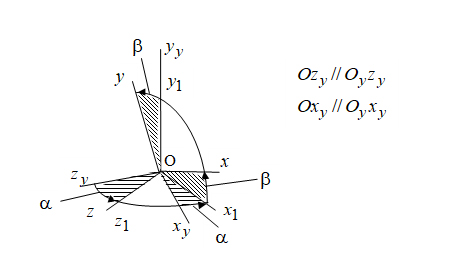
\includegraphics[]{img-18} 
		\caption{Кинематическая схема}
		\label{fig:coord/3.4}
	\end{figure}

	Ось $O_{y_1}$ направлена по оси вращения АВ, ось $O_{z_1}$ направлена по оси вращения CD, ось $O_{x_1}$ дополняет указанные оси до правой системы координат. Точка O находится на пересечении осей АВ и CD. Положение точки О в установочной системе координат определяется радиусом-вектором
	\begin{equation}
	\label{eq:p3:1}
	\begin{alignedat}{2}
	\bar{r}_0 = \bar{e}_y\tilde{r}_0,
	\end{alignedat}
	\end{equation}
	где $\tilde{r}_0 = \left( \begin{matrix}	0 & -l & 0 \end{matrix} \right)^T$.
	
	Орты осей $O_{x_1y_1z_1}$ обозначим $\bar{i}_1$, $\bar{j}_1$, $\bar{k}_1$ и составим из них базисную строку $\bar{e}_1 = (\bar{i}_1 \bar{j}_1 \bar{k}_1)$. Связь между базисными строками $\bar{e}_y$ и $\bar{e}_1$ определяются матрицей $A_1$:
	\begin{equation}
	\label{eq:p3:2}
	\begin{alignedat}{2}
	\bar{e}_y = \bar{e}_1	A_1,
	\end{alignedat}
	\end{equation}
	где \( A_{1}= \left( \begin{matrix}
	cos \alpha & 0 & -sin \alpha \\
	0 & 1 & 0\\
	sin \alpha & 0 & cos \alpha \\
	\end{matrix}
	\right) \) . 
	
	Масса 1-го тела равна \( m_{1} \), положение центра масс в системе координат \( Ox_{1}y_{1}z_{1} \) определяется радиусом-вектором 
	
	\begin{equation}
	\label{eq:p3:3}
	\begin{alignedat}{2}
	\bar{r}_{c_{1}}=\bar{e}_{1}\tilde{r}_{c_{1}},
	\end{alignedat}
	\end{equation}
	
	где \( \tilde{r}_{c_{1}}= \left( \begin{matrix}
	x_{c_{1}} & y_{c_{1}} & z_{c_{1}}\\
	\end{matrix}
	\right) ^{T} \) . 
	Введем следующие обозначения для осевых и центробежных моментов инерции 1-го тела: 
	
	\( J_{x_{1}}=A_{1},J_{y_{1}}=B_{1},J_{z_{1}}=C_{1},J_{x_{1}y_{1}}=F_{1},J_{x_{1}z_{1}}=E_{1},J_{y_{1}z_{1}}=D_{1} \), 
	
	тогда его тензор инерции 
	
	\begin{equation}
	\label{eq:p3:4}
	\begin{alignedat}{2}
	J_{1}= \left( \begin{matrix}
	A_{1} & -F_{1} & -E_{1}\\
	-F_{1} & B_{1} & -D_{1}\\
	-E_{1} & -D_{1} & C_{1}\\
	\end{matrix}
	\right) 
	\end{alignedat}
	\end{equation}
		
	\item Оси \( O_{xyz} \) (рисунок \ref{fig:coord/3.4}) жестко связаны с телом 2: ось \( O_x \) направлена по оптической оси, ось \( O_z \) совпадает с осью вращения \textit{CD}, ось \( O_y \) дополняет указанные оси до правой системы координат. 
	
	Орты осей \( O_{x_{1}y_{1}z_{1}} \) обозначим \( \bar{i},\bar{j},\bar{k}_{1} \) и составим из них базисную строку 
	\( \bar{e}= \left( \begin{matrix}	\bar{i} & \bar{j} & \bar{k}\\	\end{matrix}
	\right) \) . Связь между базисными строками \( \bar{e} \) и \( \bar{e}_{1} \) определяется матрицей \( A_{2} \): 
	
	\begin{equation}
	\label{eq:p3:5}
	\begin{alignedat}{2}
	\bar{e}_{1}=\bar{e}A_{2},
	\end{alignedat}
	\end{equation}
	
	где \( A_{2}= \left( \begin{matrix}
	cos \beta & sin \beta & 0\\
	-sin \beta & cos \beta & 0\\
	0 & 0 & 1\\
	\end{matrix}
	\right) \) . 
	
	Масса 2-го тела равна \( m_{2} \), положение центра масс в системе координат \( O_{xyz} \) определяется радиусом-вектором 
	
	\begin{equation}
	\label{eq:p3:6}
	\begin{alignedat}{2}
	\bar{r}_{c_{2}}=\bar{e} \tilde{r}_{c_{2}},
	\end{alignedat}
	\end{equation}
	
	где \( \tilde{r}_{c_{2}}= \left( \begin{matrix}
	x_{c_{2}} & y_{c_{2}} & z_{c_{2}}\\
	\end{matrix}
	\right) ^{T} \) . 
	
	Введем следующие обозначения для осевых и центробежных моментов инерции 2-го тела: 
	
	\( J_{x_{}}=A_{2},J_{y}=B_{2},J_{z}=C_{2},J_{x_{2}y_{2}}=F_{2},J_{x_{2}z_{2}}=E_{2},J_{y_{2}z_{2}}=D_{2} \), 
	
	тогда его тензор инерции 
	
	\begin{equation}
	\label{eq:p3:7}
	\begin{alignedat}{2}
	J_{2}= \left( \begin{matrix}
	A_{2} & -F_{2} & -E_{2}\\
	-F_{2} & B_{2} & -D_{2}\\
	-E_{2} & -D_{2} & C_{2}\\
	\end{matrix}
	\right) 
	\end{alignedat}
	\end{equation}	
	\item Движение ЛА происходит в однородном поле силы тяжести.
\end{enumerate}


\subsection{Геометрия масс} \label{sec:ch3/sec4}

По рабочим чертежам в среде Solid Works получены массовые характеристики ОУ. Их обозначения и величины приведены в таблице ниже (таблица \ref{tab:MASS/3.1}).



{
	\setlength\extrarowheight{3pt}
	\begin{longtable}{p{0.66in}p{1.94in}p{0.71in}p{0.29in}p{0.49in}p{0.39in}p{0.66in}}
		\caption{Массовые характеристики ОУ}%
		\label{tab:MASS/3.1}% label всегда желательно идти после caption
		\\
\hline
		%row no:1
		\multicolumn{1}{|p{0.66in}}{№ п/п} & 
		\multicolumn{1}{|p{1.94in}}{Наименование} & 
		\multicolumn{1}{|p{0.71in}}{Обозна-\par чение} & 
		\multicolumn{3}{|p{1.57in}}{Величина} & 
		\multicolumn{1}{|p{0.66in}|}{Размер-\par ность} \\
		\hline
		%row no:2
		\multicolumn{1}{|p{0.66in}}{1} & 
		\multicolumn{1}{|p{1.94in}}{2} & 
		\multicolumn{1}{|p{0.71in}}{3} & 
		\multicolumn{3}{|p{1.57in}}{4} & 
		\multicolumn{1}{|p{0.66in}|}{5} \\
		\hline
		%row no:3
		\multicolumn{1}{|p{0.66in}}{1} & 
		\multicolumn{1}{|p{1.94in}}{Координаты центра прибора относительно центра масс носителя } & 
		\multicolumn{1}{|p{0.71in}}{Y\textsubscript{0} \par X\textsubscript{0} \par Z\textsubscript{0}} & 
		\multicolumn{1}{|p{0.29in}}{-0.5 -0.5 -2} & 
		\multicolumn{1}{|p{0.49in}}{0 -8.422 0} & 
		\multicolumn{1}{|p{0.39in}}{-0.5 -0.5 2} & 
		\multicolumn{1}{|p{0.66in}|}{\textit{м}} \\
		\hline
		%row no:4
		\multicolumn{1}{|p{0.66in}}{2} & 
		\multicolumn{1}{|p{1.94in}}{\multirowcell{2}{}{\begin{tabular}{p{1.94in}}Масса 1-го тела вращения (по азимуту),  \\\end{tabular}}} & 
		\multicolumn{1}{|p{0.71in}}{m\textsubscript{1}} & 
		\multicolumn{3}{|p{1.57in}}{15.7} & 
		\multicolumn{1}{|p{0.66in}|}{\textit{кг}} \\
		\hline
		%row no:5
		\multicolumn{1}{|p{0.66in}}{3} & 
		\multicolumn{1}{|p{1.94in}}{координаты его центра масс} & 
		\multicolumn{1}{|p{0.71in}}{x\textsubscript{C1}} & 
		\multicolumn{3}{|p{1.57in}}{-2.82} & 
		\multicolumn{1}{|p{0.66in}|}{\textit{мм}} \\
		\hline
		%row no:6
		\multicolumn{1}{|p{0.66in}}{4} & 
		\multicolumn{1}{|p{1.94in}}{} & 
		\multicolumn{1}{|p{0.71in}}{z\textsubscript{C1}} & 
		\multicolumn{3}{|p{1.57in}}{8.64} & 
		\multicolumn{1}{|p{0.66in}|}{\textit{мм}} \\
		\hline
		%row no:7
		\multicolumn{1}{|p{0.66in}}{5} & 
		\multicolumn{1}{|p{1.94in}}{} & 
		\multicolumn{1}{|p{0.71in}}{y\textsubscript{C1}} & 
		\multicolumn{3}{|p{1.57in}}{-95.03} & 
		\multicolumn{1}{|p{0.66in}|}{\textit{мм}} \\
		\hline
		%row no:8
		\multicolumn{1}{|p{0.66in}}{6} & 
		\multicolumn{1}{|p{1.94in}}{осевые моменты инерции (Ось вращения – Y)} & 
		\multicolumn{1}{|p{0.71in}}{ \( J_{x_{1}}=A_{1} \) } & 
		\multicolumn{3}{|p{1.57in}}{212} & 
		\multicolumn{1}{|p{0.66in}|}{\textit{гр м\textsuperscript{2}}} \\
		\hline
		%row no:9
		\multicolumn{1}{|p{0.66in}}{7} & 
		\multicolumn{1}{|p{1.94in}}{} & 
		\multicolumn{1}{|p{0.71in}}{ \( J_{y_{1}}=B_{1} \) } & 
		\multicolumn{3}{|p{1.57in}}{311.8} & 
		\multicolumn{1}{|p{0.66in}|}{\textit{гр м\textsuperscript{2}}} \\
		\hline
		%row no:10
		\multicolumn{1}{|p{0.66in}}{12} & 
		\multicolumn{1}{|p{1.94in}}{\multirowcell{2}{}{\begin{tabular}{p{1.94in}}Масса 2-го тела вращения (по углу места),  \\\end{tabular}}} & 
		\multicolumn{1}{|p{0.71in}}{ \( m_{2} \) } & 
		\multicolumn{3}{|p{1.57in}}{1130.85} & 
		\multicolumn{1}{|p{0.66in}|}{\textit{гр}} \\
		\hline
		%row no:11
		\multicolumn{1}{|p{0.66in}}{13} & 
		\multicolumn{1}{|p{1.94in}}{координаты его центра масс,} & 
		\multicolumn{1}{|p{0.71in}}{ \( x_{C_{2}} \) } & 
		\multicolumn{3}{|p{1.57in}}{0} & 
		\multicolumn{1}{|p{0.66in}|}{\textit{мм}} \\
		\hline
		%row no:12
		\multicolumn{1}{|p{0.66in}}{14} & 
		\multicolumn{1}{|p{1.94in}}{} & 
		\multicolumn{1}{|p{0.71in}}{ \( y_{C_{2}} \) } & 
		\multicolumn{3}{|p{1.57in}}{14.8} & 
		\multicolumn{1}{|p{0.66in}|}{\textit{мм}} \\
		\hline
		%row no:13
		\multicolumn{1}{|p{0.66in}}{15} & 
		\multicolumn{1}{|p{1.94in}}{} & 
		\multicolumn{1}{|p{0.71in}}{ \( z_{C_{2}} \) } & 
		\multicolumn{3}{|p{1.57in}}{-8} & 
		\multicolumn{1}{|p{0.66in}|}{\textit{мм}} \\
		\hline
		%row no:14
		\multicolumn{1}{|p{0.66in}}{16} & 
		\multicolumn{1}{|p{1.94in}}{осевые моменты инерции (Ось вращения - Z)} & 
		\multicolumn{1}{|p{0.71in}}{ \( J_{x_{2}}=A_{2} \) } & 
		\multicolumn{3}{|p{1.57in}}{3.3} & 
		\multicolumn{1}{|p{0.66in}|}{\textit{гр м\textsuperscript{2}}} \\
		\hline
		%row no:15
		\multicolumn{1}{|p{0.66in}}{17} & 
		\multicolumn{1}{|p{1.94in}}{} & 
		\multicolumn{1}{|p{0.71in}}{ \( J_{y_{2}}=B_{2} \) } & 
		\multicolumn{3}{|p{1.57in}}{7.5} & 
		\multicolumn{1}{|p{0.66in}|}{\textit{гр м\textsuperscript{2}}} \\
		\hline
		%row no:16
		\multicolumn{1}{|p{0.66in}}{18} & 
		\multicolumn{1}{|p{1.94in}}{} & 
		\multicolumn{1}{|p{0.71in}}{ \( J_{z_{2}}=C_{2} \) } & 
		\multicolumn{3}{|p{1.57in}}{8.4} & 
		\multicolumn{1}{|p{0.66in}|}{\textit{гр м\textsuperscript{2}}} \\
		\hline
		
\end{longtable}}

%%%%%%%%%%%%%%%%%%%% Table No: 4 ends here %%%%%%%%%%%%%%%%%%%%

\section{Составление уравнений динамической модели ОУ} \label{ch:ch3/sect5}

ОУ моделируется двумя абсолютно твердыми телами (тело 1 и тело 2), установленными в корпусе, который закреплен на ЛА. Положение этих тел относительно корпуса однозначно определяется углами поворотов: \( \alpha \) и \( \beta \) . К активным силам, действующим на ОЭП, отнесем силы тяжести, момент от азимутального привода – моментного двигателя, момент от угломестного привода – второго моментного двигателя, моменты трения. Тогда связи, ограничивающие перемещения указанных тел, можно считать идеальными. Кроме того, связи являются голономными, удерживающими и стационарными. Для построения математической модели относительного движения ОУ в установочной системе координат (движения относительно корпуса) будем использовать уравнения Лагранжа II-го рода. Метод их составления для относительного движения объекта, установленного на подвижном основании, описан в разделе \ref{ch:ch3/sect1}. Механическая модель. Он состоит из трех этапов: вычисления кинетической энергии, вычисления обобщенных сил и составления уравнений движения (проведения действий в соответствии с уравнениями Лагранжа II-го рода). За обобщенные координаты принимаются углы поворота: \( q_{1}= \alpha, q_{2}= \beta \) . 





\subsection{Вычисление кинетической энергии} \label{sec:ch3/sec6}

Вычислим кинетическую энергию ОУ, находящемся на ЛА, совершающем произвольный маневр, в соответствии с уравнениями (\labelcref{eq:p3:1}). Вектор ускорения центра масс ЛА, вектор угловой скорости и вектор углового ускорения определяются соответственно выражениями (\labelcref{eq:p3:5,eq:p3:6,eq:p3:7}). Будем учитывать вибрацию установочной системы координат, которая задается уравнениями (\labelcref{eq:p3:9}).

Кинетическая энергия ОЭС в относительном движении в установочных осях \( Ox_{y}y_{y}z_{y} \) (тело 1 совершает вращательное движение, тело 2 – сферическое) определяется следующим образом: 

\begin{equation}
\label{eq:p3:8}
\begin{alignedat}{2}
T_{r}= 
\sum_{j=1}^{2}T_{r}^{ \left( j \right) }= 
\sum_{j=1}^{2}\frac{1}{2} \left( \tilde{\omega}_{j}^{r} \right) ^{T}J_{j} \tilde{\omega}_{j}^{r}
\end{alignedat}
\end{equation}

здесь 
\( J_{j} \) – тензор инерции и 
\( \tilde{\omega}_{j}^{r} \) – координатный вектор относительной угловой скорости \textit{j}–го тела в системе координат, связанной с этим телом. 


Векторы угловых скоростей 1-го и 2-го тел в установочной системе координат \( Ox_{y}y_{y}z_{y} \) определяются в соответствии с изображением систем координат (рисунок~\ref{fig:coord/3.4}). Угловая скорость 1-го тела 

\begin{equation}
\label{eq:p3:9}
\begin{alignedat}{2}
\bar{\omega}_{1}^{r}=e_{1} \tilde{\omega}_{1}^{r}=e_{1} \left( \begin{matrix}
0\\
\dot{\alpha} \\
0\\
\end{matrix}
\right),
\end{alignedat}
\end{equation}

угловая скорость 2-го тела 

\begin{equation}
\label{eq:p3:10}
\begin{alignedat}{2}
 \bar{\omega}_{2}^{r}=\bar{e}_{2} \tilde{\omega}_{2}^{r}=\bar{e}_{2} \left( \begin{matrix}
\dot{\alpha} sin \beta \\
\dot{\alpha} cos \beta \\
\dot{\beta} \\
\end{matrix}
\right) .
\end{alignedat}
\end{equation}

С учетом принятых обозначений (\labelcref{eq:p3:4}) и (\labelcref{eq:p3:7}), а также выражений (\labelcref{eq:p3:9}),(\labelcref{eq:p3:10}), после проведения действий в соответствии с (\labelcref{eq:p3:8}) находим 

\begin{equation}
\label{eq:p3:11}
\begin{alignedat}{2}
T_{r}=
\frac{1}{2} 
[ 
	( 
		B_{1}+
		A_{2}sin^{2} ( \beta ) +
		B_{2}cos^{2} ( \beta ) -
		F_{2}sin ( 2 \beta ) 
	) \dot{\alpha}^{2} + \\
	C_{2} \dot{\beta}^{2} - 
	2 ( 
		E_{2}sin ( \beta ) +
		D_{2}cos ( \beta ) 
	) 
	\dot{\alpha} \dot{\beta} 
] 
\end{alignedat}
\end{equation}

Кинетический момент ОУ относительно точки \textit{О} в относительном движении в установочных осях \( Ox_{y}y_{y}z_{y} \) равен 

\begin{equation}
\label{eq:p3:12}
\begin{alignedat}{2}
\bar{K}_{O}^{r}= \sum_{j=1}^{2}\bar{e}_{j}J_{j} \tilde{\omega}_{j}^{r}
\end{alignedat}
\end{equation}

Из выражений (\labelcref{eq:p3:2}), (\labelcref{eq:p3:5}), учитывая то, что матрицы в этих выражениях являются ортогональными, имеем 

\begin{equation}
\label{eq:p3:13}
\begin{alignedat}{2}
\bar{e}_{1} = \bar{e}_{y} A_{1}^{T},
\bar{e}_{2} = 
\bar{e} = 
\bar{e}_{1}A_{2}^{T} = 
e_{y}A_{1}^{T}A_{2}^{T},
\end{alignedat}
\end{equation}

Тогда 

\begin{equation}
\label{eq:p3:14}
\begin{alignedat}{2}
\bar{K}_{O}^{r}=\bar{e}_{y} [ 
	A_{1}^{T}J_{1} \tilde{\omega}_{1}^{r} + A_{1}^{T} A_{2}^{T} J_{2} \tilde{\omega}_{2}^{r} 
] 
\end{alignedat}
\end{equation}

С учетом принятых обозначений (\labelcref{eq:p3:4}),(\labelcref{eq:p3:7}) и выражений (\labelcref{eq:p3:9}),(\labelcref{eq:p3:10}), после проведения действий в соответствии с (\labelcref{eq:p3:14}) получим 

\begin{equation}
\label{eq:p3:15}
\begin{alignedat}{2}
\bar{K}_{O}^{r}=\bar{e}_{y}\tilde{K}_{O}^{r}=\bar{e}_{y} \left( \begin{matrix}
K_{x_{y}}^{r} \left( q,\dot{q} \right) \\
K_{y_{y}}^{r} \left( q,\dot{q} \right) \\
K_{z_{y}}^{r} \left( q,\dot{q} \right) \\
\end{matrix}
\right) 
\end{alignedat}
\end{equation}

где 

\( q= \left( \begin{matrix}
\alpha \\
\beta \\
\end{matrix}
\right) \),\ \ \ \( \dot{q}= \left( \begin{matrix}
\dot{\alpha} \\
\dot{\beta} \\
\end{matrix}
\right) \), 
\begin{equation}
\begin{multlined}
K_{x_{y}}^{r} ( q,\dot{q} ) = 
[
	-( 
		F_{1}cos ( \alpha ) +
		D_{1}sin ( \alpha ) 
	) + \nonumber \\
	( 
		\frac{A_{2}-B_{2}}{2}sin ( 2 \beta ) -
		F_{2}cos ( 2 \beta ) 
	) cos ( \alpha ) \nonumber \\
	- ( 
		E_{2}sin ( \beta ) +
		D_{2}cos ( \beta ) 
	) sin ( \alpha ) 
] \dot{\alpha} + \nonumber \\
[
	- ( 
		E_{2}cos ( \beta ) -
		D_{2}sin ( \beta ) 
	) cos ( \alpha ) +
	C_{2}sin ( \alpha ) 
] \dot{\beta}	,\nonumber
\end{multlined}
\end{equation}

\begin{equation}
\begin{multlined}
 K_{y_{y}}^{r} \left( q,\dot{q} \right) = 
 [ B_{1}+A_{2}sin^{2} ( \beta ) +B_{2}cos^{2} ( \beta ) -F_{2}sin ( 2 \beta ) ] \dot{\alpha} - \nonumber \\
 ( E_{2}sin ( \beta ) +D_{2}cos ( \beta ) ) \beta, \nonumber
\end{multlined}
\end{equation}

\begin{equation}
\begin{multlined}
K_{z_{y}}^{r} \left( q,\dot{q} \right) = 
[ 
	\left( F_{1}sin ( \alpha ) -D_{1}cos ( \alpha ) \right) - \nonumber \\
	\left( \frac{A_{2}-B_{2}}{2}sin ( 2 \beta ) -F_{2}cos ( 2 \beta ) \right) sin ( \alpha ) - \nonumber \\
	\left( E_{2}sin ( \beta ) +D_{2}cos ( \beta ) \right) cos ( \alpha )
]
\dot{\alpha} + \nonumber \\
[ 
	- \left( E_{2}cos ( \beta ) -D_{2}sin ( \beta ) \right) sin ( \alpha ) +C_{2}cos ( \alpha ) 
] 
\dot{\beta} \nonumber
\end{multlined}
\end{equation}

Вектор угловой скорости установочной системы координат \( O_{x_{y}y_{y}z_{y}} \) в системе координат \( O_{XYZ} \) \ (переносного движения) определяется суммой угловых скоростей ЛА и вибрацией установочной системы координат: 






\begin{equation} % %\tag{3.16}
\label{eq:p3:16}
\begin{multlined}
\bar{\omega} = 
\bar{\omega}_{\textit{ЛА}}+ \bar{\omega}_{\textit{вибр}}=
\bar{e}_{c} \tilde{\omega}_{c}+\bar{e}_{\textit{y}} \tilde{\omega}_{\textit{вибр}}=
\bar{e}_{y} \left( A_{y} \tilde{\omega}_{c}+ \tilde{\omega}_{\textit{вибр}} \right) = \\
\bar{e}_{y} \omega =\bar{e}_{y} \left( \begin{matrix}
\omega_{x_{y}} & \omega_{y_{y}} & \omega_{z_{y}}\\
\end{matrix}
\right) ^{T}.
\end{multlined}
\end{equation}
С учетом (\labelcref{eq:p3:15}) и (\labelcref{eq:p3:16}) определим кинетическую энергию 


\begin{equation} % %\tag{3.17}
\label{eq:p3:17}
T_{e}= 
\sum_{j=1}^{2} \bar{\omega} \left( \bar{K}_{O}^{r} \right)^{ \left( j \right) }= 
\bar{\omega} \bar{K}_{O}^{r}= 
\tilde{\omega}^{T}\tilde{K}_{O}^{r}= 
\omega_{x_{y}}K_{x_{y}}^{r}+ \omega_{y_{y}}K_{y_{y}}^{r}+ \omega_{z_{y}}K_{z_{y}}^{r}
\end{equation}
Вычислим составляющую кинетической энергии 


\begin{equation} % %\tag{3.18}
\label{eq:p3:18}
T^{\ast}= \sum_{j=1}^{2}\frac{1}{2} \tilde{\omega}_{j}^{T}J^{ \left( j \right) } \tilde{\omega}_{j}
\end{equation}
Запишем вектор угловой скорости переносного движения в базисах, связанных с 1–м, 2–м телами: 


\begin{equation} % %\tag{3.19}
\label{eq:p3:19}
\bar{\omega} =\bar{e}_{y} \tilde{\omega} =\bar{e}_{1}A_{1} \tilde{\omega} =\bar{e}_{2}A_{2} \tilde{\omega} 
\end{equation}
С учетом (\labelcref{eq:p3:19}) выражение (\labelcref{eq:p3:18}) запишется в следующем виде 


\begin{equation} % %\tag{3.20}
\label{eq:p3:20}
T^{\ast}=
\frac{1}{2} \tilde{\omega} ^{T} [ A_{1}^{T} ( J^{ ( 1 ) }+A_{2}^{T}J^{ ( 2 ) }A_{2} ) A_{1} ] \tilde{\omega}
\end{equation}
Обозначим 


\begin{equation} % %\tag{3.21}
\label{eq:p3:21}
J \left( \beta \right) = \left( J_{1}+A_{2}^{T}J_{2}A_{2} \right) 
\end{equation}
Матрица \( J \left( \beta \right) \) является симметрической, введем следующие обозначения для ее элементов 


\begin{equation} % %\tag{3.22}
\label{eq:p3:22}
J \left( \beta \right) = \left( \begin{matrix}
A_{1}+A \left( \beta \right) & -F_{1}-F \left( \beta \right) & -E_{1}-E \left( \beta \right) \\
-F_{1}-F \left( \beta \right) & B_{1}+B \left( \beta \right) & -D_{1}-D \left( \beta \right) \\
-E_{1}-E \left( \beta \right) & -D_{1}-D \left( \beta \right) & C_{1}+C_{2}\\
\end{matrix}
\right) 
\end{equation}
где 

\( A \left( \beta \right) =A_{2}cos^{2} \left( \beta \right) +B_{2}sin^{2} \left( \beta \right) +F_{2}sin \left( 2 \beta \right) \), 

\( F \left( \beta \right) =F_{2}cos \left( 2 \beta \right) -\frac{A_{2}-B_{2}}{2}sin \left( 2 \beta \right) \), 

\( E \left( \beta \right) =E_{2}cos \left( \beta \right) -D_{2}sin \left( \beta \right) \), 

\( B \left( \beta \right) =B_{2}cos^{2} \left( \beta \right) +A_{2}sin^{2} \left( \beta \right) -F_{2}sin \left( 2 \beta \right) \), 

\( D \left( \beta \right) =D_{2}cos \left( \beta \right) +E_{2}sin \left( \beta \right) \) . 

Обозначим 

\begin{equation} % %\tag{3.23}
\label{eq:p3:23}
J \left( \alpha, \beta \right) =A_{1}^{T} \left( J_{1}+A_{2}^{T}J_{2}A_{2} \right) A_{1}
\end{equation}
Матрица \( J \left( \alpha, \beta \right) \) является симметрической, введем следующие обозначения для ее элементов 


\begin{equation} % %\tag{3.24}
\label{eq:p3:24}
J \left( \alpha, \beta \right) = \left( \begin{matrix}
A \left( \alpha, \beta \right) & -F \left( \alpha, \beta \right) & -E \left( \alpha, \beta \right) \\
-F \left( \alpha, \beta \right) & B_{1}+B \left( \beta \right) & -D \left( \alpha, \beta \right) \\
-E \left( \alpha, \beta \right) & -D \left( \alpha, \beta \right) & C \left( \alpha, \beta \right) \\
\end{matrix}
\right) 
\end{equation}
где 
\begin{equation}
\begin{multlined}
 A ( \alpha, \beta ) = 
 ( A_{1}+A ( \beta ) ) cos^{2} ( \alpha ) + 
 ( C_{1}+C_{2} ) sin^{2} ( \alpha ) - \nonumber \\
 ( E_{1}+E ( \beta ) ) sin ( 2 \alpha ),\nonumber \\
\end{multlined}
\end{equation}
\begin{equation}
\begin{multlined}
 F \left( \alpha, \beta \right) = \left( F_{1}+F \left( \beta \right) \right) cos \left( \alpha \right) + \left( D_{1}+D \left( \beta \right) \right) sin \left( \alpha \right),\nonumber \\
\end{multlined}
\end{equation}
\begin{equation}
\begin{multlined}
 E \left( \alpha, \beta \right) =\frac{A_{1}+A \left( \beta \right) -C_{1}-C_{2}}{2}sin \left( 2 \alpha \right) + \left( E_{1}+E \left( \beta \right) \right) cos \left( 2 \alpha \right),\nonumber \\
\end{multlined}
\end{equation}
\begin{equation}
\begin{multlined}
 D \left( \alpha, \beta \right) = \left( D_{1}+D \left( \beta \right) \right) cos \left( \alpha \right) - \left( F_{1}+F \left( \beta \right) \right) sin \left( \alpha \right),\ \nonumber \\
\end{multlined}
\end{equation}
\begin{equation}
\begin{multlined}
 C \left( \alpha, \beta \right) = \left( C_{1}+C_{2} \right) cos^{2} \left( \alpha \right) + \left( A_{1}+A \left( \beta \right) \right) sin^{2} \left( \alpha \right) + \left( E_{1}+E \left( \beta \right) \right) sin \left( 2 \alpha \right) . \nonumber \\
\end{multlined}
\end{equation}
Используя обозначения (\labelcref{eq:p3:24}), выражение (\labelcref{eq:p3:20}) для кинетической энергии запишется в следующем виде: 


\begin{equation} % %\tag{3.25}
\label{eq:p3:25}
\begin{multlined}
T^{\ast}=
\frac{1}{2} 
[ 
	A ( \alpha, \beta ) \omega_{x_{y}}^{2} ( t ) + 
	( B_{1}+B ( \beta ) ) \omega_{y_{y}}^{2} ( t ) +
	C ( \alpha, \beta ) \omega_{z_{y}}^{2} ( t ) - \\
	2F ( \alpha, \beta ) \omega_{x_{y}} ( t ) \omega_{y_{y}} ( t ) -
	2E ( \alpha, \beta ) \omega_{x_{y}} ( t ) \omega_{z_{y}} ( t ) -
	2D ( \alpha, \beta ) \omega_{y_{y}} ( t ) \omega_{z_{y}} ( t ) 
] .
\end{multlined}
\end{equation}
С учетом введенных обозначений (\labelcref{eq:p3:22}) выражение для кинетической энергии (\labelcref{eq:p3:11}) запишется компактнее: 


\begin{equation} % %\tag{3.26}
\label{eq:p3:26}
T_{r}=
\frac{1}{2} 
[ 
	( B_{1}+B ( \beta ) ) \dot{\alpha}^{2}+
	C_{2} \dot{\beta}^{2} - 
	2D \left( \beta \right) \dot{\alpha} \dot{\beta} 
]
\end{equation}
С учетом обозначений (\labelcref{eq:p3:22}) и (\labelcref{eq:p3:24}) выражения для проекций кинетического момента \( K_{O}^{r} \) (\labelcref{eq:p3:15}) запишутся компактнее: 

\( 
K_{x_{y}}^{r} ( q,\dot{q} ) =
-F ( \alpha, \beta ) \dot{\alpha} - 
[ 
	E ( \beta ) cos ( \alpha ) - 
	C_{2}sin ( \alpha ) 
] \dot{\beta} 
\), 

\( 
K_{y_{y}}^{r} ( q,\dot{q} ) = 
[ B_{1}+B \left( \beta \right) ] \dot{\alpha} -
D ( \beta ) \dot{\beta} 
\), 

\( 
K_{z_{y}}^{r} ( q,\dot{q} ) =
-D ( \alpha, \beta ) \dot{\alpha} + 
[ 
E ( \beta ) sin ( \alpha ) +
C_{2}cos ( \alpha ) 
] \dot{\beta} 
\), 

и выражение для кинетической энергии (\labelcref{eq:p3:17}) запишется следующим образом:


\begin{equation} % %\tag{3.27}
\label{eq:p3:27}
\begin{multlined}
T_{e}= 
	\omega_{x_{y}} ( t ) 
	[ 
		-F ( \alpha, \beta ) \dot{\alpha} - 
		( 
			E ( \beta ) cos ( \alpha ) -
			C_{2}sin ( \alpha ) 
		) 
		\dot{\beta } 
	] + \\
	+ \omega_{y_{y}} ( t ) 
	[ 
		( B_{1}+B ( \beta ) ) 
		\dot{\alpha} -
		D ( \beta ) \dot{\beta } 
	] + \\
	\omega_{z_{y}} ( t ) 
	[ 
		-D ( \alpha, \beta ) \dot{\alpha} + 
		( 
			E ( \beta ) sin ( \alpha ) +
			C_{2}cos ( \alpha ) 
		) \dot{\beta } 
	] 
\end{multlined}
\end{equation}

В соответствии с (\labelcref{eq:p3:23}), используя выражения (\labelcref{eq:p3:25,eq:p3:27}), получим

\begin{equation} % %\tag{3.28}
\label{eq:p3:28}
\begin{multlined}
T=\frac{1}{2} 
\left\lbrace 
	( B_{1}+B ( \beta ) ) \dot{\alpha}^{2}+
	C_{2} \dot{\beta} ^{2} - 
	2D ( \beta ) \dot{\alpha} \dot{\beta} 
\right\rbrace + \\ 
\omega_{x_{y}} ( t ) 
[ 
	-F ( \alpha, \beta ) \dot{\alpha} - 
	(
		E ( \beta ) cos ( \alpha ) -
		C_{2}sin ( \alpha ) 
	) \beta 
] + \\
\omega_{y_{y}} ( t ) 
[ 
	( B_{1}+B ( \beta ) ) \dot{\alpha} -
	D ( \beta ) \dot{\beta} 
] + \\
\omega_{z_{y}} ( t ) 
[ 
	-D ( \alpha, \beta ) \dot{\alpha} + 
	( E ( \beta ) sin ( \alpha ) +C_{2}cos ( \alpha ) ) \dot{\beta} 
] + \\
\frac{1}{2} 
[
	A ( \alpha, \beta ) \omega_{x_{y}}^{2} ( t ) + 
	( B_{1}+B ( \beta ) ) \omega_{y_{y}}^{2} ( t ) + \\
	C ( \alpha, \beta ) \omega_{z_{y}}^{2} ( t ) - 
	2F ( \alpha, \beta ) \omega_{x_{y}} ( t ) \omega_{y_{y}} ( t ) - \\
	2E ( \alpha, \beta ) \omega_{x_{y}} ( t ) \omega_{z_{y}} ( t ) -
	2D ( \alpha, \beta ) \omega_{y_{y}} ( t ) \omega_{z_{y}} ( t ) 
].
\end{multlined}
\end{equation}
Выражение (\labelcref{eq:p3:25,eq:p3:28}) определяет кинетическую энергию ОУ с учетом движения носителя и с учетом вибрации. 

\subsection{Вычисление обобщенных сил} \label{sec:ch3/sec7}

Для вычисления составляющих обобщенных сил, характеризующих действие переносных сил инерции (\labelcref{eq:p3:22}), нужно знать ускорение точки \textit{О}. Силы (\labelcref{eq:p3:22}) вызывают появление обобщенных сил 

\begin{equation} %\tag{3.29}
\label{eq:p3:29}
\begin{multlined}
Q_{i}^{`}= 
\sum _{j=1}^{2} \sum _{k=1}^{\infty} \left( -m_{k}^{ \left( j \right) }\bar{a}_{0} \frac{ \partial \bar{r}_{k}^{ \left( j \right) }}{ \partial q_{i}} \right) = 
\sum _{j=1}^{2} \sum _{k=1}^{\infty} \left( -\bar{a}_{0} \frac{ \partial \left( m_{k}^{ \left( j \right) }\bar{r}_{k}^{ \left( j \right) } \right) }{ \partial q_{i}} \right) = \\
- \sum _{j=1}^{2}\bar{a}_{0} \left( \frac{ \partial \left( \sum _{k=1}^{\infty} \left( m_{k}^{ \left( j \right) }\bar{r}_{k}^{ \left( j \right) } \right) \right) }{ \partial q_{i}} \right) =
- \sum _{j=1}^{2} \left( m_{j}\bar{a}_{0} \frac{ \partial \bar{r}_{C}^{ \left( j \right) }}{ \partial q_{i}} \right) \left( i=1,2 \right),
\end{multlined}
\end{equation}
здесь \( \bar{r}_{C}^{ \left( j \right) } \) –\ радиус-вектор центра масс \textit{j-}го\ тела в системе координат \( Ox_{y}y_{y}z_{y} \), \( m_{j} \) – масса \textit{j - }го тела, \( q_{i} \) – \textit{i}–я обобщенная координата. 

Запишем радиусы-векторы центров масс 1–го и 2–го тел в базисе установочной системы координат: 


\begin{equation} %\tag{3.30}
\label{eq:p3:30}
\begin{multlined}
\bar{r}_{C_{1}}=\bar{e}_{1}\tilde{r}_{C_{1}}=\bar{e}_{y}A_{1}^{T}\tilde{r}_{C_{1}}=\bar{e}_{y} \left( \begin{matrix}
x_{C_{1}}cos \left( \alpha \right) +z_{C_{1}}sin \left( \alpha \right) \\
y_{C_{1}}\\
-x_{C_{1}}sin \left( \alpha \right) +z_{C_{1}}cos \left( \alpha \right) \\
\end{matrix}
\right) 
\end{multlined}
\end{equation}

\begin{equation} %\tag{3.31}
\label{eq:p3:31}
\begin{multlined}
\bar{r}_{C_{2}}=\bar{e}\tilde{r}_{C_{2}}=\bar{e}_{y}A_{1}^{T}A_{2}^{T}\tilde{r}_{C_{2}}=\bar{e}_{y} \left( \begin{matrix}
\left( x_{C_{2}}cos \left( \beta \right) -y_{C_{2}}sin \left( \beta \right) \right) cos \left( \alpha \right) +z_{C_{2}}sin \left( \alpha \right) \\
x_{C_{2}}sin \left( \beta \right) +y_{C_{2}}cos \left( \beta \right) \\
- \left( x_{C_{2}}cos \left( \beta \right) -y_{C_{2}}sin \left( \beta \right) \right) sin \left( \alpha \right) +z_{C_{2}}cos \left( \alpha \right) \\
\end{matrix}
\right) 
\end{multlined}
\end{equation}
В соответствии с выражением (\labelcref{eq:p3:29}) находим

\begin{equation} %\tag{3.32}
\label{eq:p3:32}
\begin{multlined}
Q_{ \alpha }^{'}=
-\tilde{a}_{O}^{T} ( t ) 
[ 
m_{1} \left( 
\begin{matrix}
	-x_{C_{1}}sin ( \alpha ) +z_{C_{1}}cos ( \alpha ) \\
	0\\
	-x_{C_{1}}cos \phi _{1}-z_{C_{1}}sin ( \alpha ) \\
\end{matrix}
\right) + \\ 
 m_{2} 
\left( 
\begin{matrix}
	- ( x_{C_{2}}cos ( \beta ) -y_{C_{2}}sin ( \beta ) ) sin ( \alpha ) +z_{C_{2}}cos ( \alpha ) \\
	0 \\
	- ( x_{C_{2}}cos ( \beta ) -y_{C_{2}}sin ( \beta ) ) cos ( \alpha ) -z_{C_{2}}sin ( \alpha ) \\
\end{matrix} 
\right) 
],
\end{multlined}
\end{equation}

\begin{equation} %\tag{3.33}
\label{eq:p3:33}
\begin{multlined}
Q_{ \beta }^{'}=-\tilde{a}_{O}^{T} \left( t \right) m_{2} \left( \begin{matrix}
\left( -x_{C_{2}}sin \left( \beta \right) -y_{C_{2}}cos \left( \beta \right) \right) cos \left( \alpha \right) \\
x_{C_{2}}cos \left( \beta \right) -y_{C_{2}}sin \left( \beta \right) \\
\left( x_{C_{2}}sin \left( \beta \right) +y_{C_{2}}cos \left( \beta \right) \right) sin \left( \alpha \right) \\
\end{matrix}
\right) 
\end{multlined}
\end{equation}

Определим составляющие обобщенных сил, характеризующие действие сил тяжести, 


\begin{equation} %\tag{3.34}
\label{eq:p3:34}
\begin{multlined}
Q_{i}^{ \left( p \right) }= \sum _{j=1}^{2} \left( m_{j}g \frac{ \partial \bar{r}_{C}^{ \left( j \right) }}{ \partial q_{i}} \right),
\end{multlined}
\end{equation}
Здесь 


\begin{equation} %\tag{3.35}
\label{eq:p3:35}
\begin{multlined}
\bar{g}=\bar{e}_{a}\tilde{g}=\bar{e}_{y}A_{y}A_{c}\tilde{g}=-\bar{e}_{y}A_{y}A_{c} \left( \begin{matrix}
0\\
g\\
0\\
\end{matrix}
\right) 
\end{multlined}
\end{equation}
Используя выражения (\labelcref{eq:p3:30}),(\labelcref{eq:p3:31}),(\labelcref{eq:p3:35}), в соответствии с (\labelcref{eq:p3:34}) находим 


\begin{equation} %\tag{3.36}
\label{eq:p3:36}
\begin{multlined}
Q_{ \alpha }^{ \left( p \right) }=
-\tilde{g}^{T}A_{c}^{T}A_{y}^{T} 
[ 
m_{1} \left( 
\begin{matrix}
	-x_{C_{1}}sin \left( \alpha \right) +z_{C_{1}}cos \left( \alpha \right) \\
	0\\
	-x_{C_{1}}cos \phi _{1}-z_{C_{1}}sin \left( \alpha \right) \\
\end{matrix}
\right) + \\
m_{2} \left( 
\begin{matrix}
	- \left( x_{C_{2}}cos \left( \beta \right) -y_{C_{2}}sin \left( \beta \right) \right) sin \left( \alpha \right) +z_{C_{2}}cos \left( \alpha \right) \\
	0\\
	- \left( x_{C_{2}}cos \left( \beta \right) -y_{C_{2}}sin \left( \beta \right) \right) cos \left( \alpha \right) -z_{C_{2}}sin \left( \alpha \right) \\
\end{matrix}
\right) 
],
\end{multlined}
\end{equation}

\vspace{\baselineskip}

\begin{equation} %\tag{3.37}
\label{eq:p3:37}
\begin{multlined}
Q_{ \beta }^{ \left( p \right) }=-\tilde{g}^{T}A_{c}^{T}A_{y}^{T}m_{2} \left( \begin{matrix}
\left( -x_{C_{2}}sin \left( \beta \right) -y_{C_{2}}cos \left( \beta \right) \right) cos \left( \alpha \right) \\
x_{C_{2}}cos \left( \beta \right) -y_{C_{2}}sin \left( \beta \right) \\
\left( x_{C_{2}}sin \left( \beta \right) +y_{C_{2}}cos \left( \beta \right) \right) sin \left( \alpha \right) \\
\end{matrix}
\right) 
\end{multlined}
\end{equation}
Составляющие обобщенных сил, определяющие воздействие приводов и моментов трения, находим, используя метод замораживания: 


\begin{equation} %\tag{3.38}
\label{eq:p3:38}
\begin{multlined}
Q_{ \alpha }^{ \left( M \right) }=\frac{ \delta A^{ \left( \alpha \right) }}{ \delta \alpha }=M_{\textit{дв.1}}-M_{\textit{тр.1}}sign \left( \alpha \right) 
\end{multlined}
\end{equation}
здесь \( M_{\textit{дв.1}} \) – момент двигателя азимутального привода, 

\( M_{\textit{тр.1}} \) – величина момента трения относительно оси вращения \textit{АВ}. 


\begin{equation} %\tag{3.39}
\label{eq:p3:39}
\begin{multlined}
Q_{ \beta }^{ \left( M \right) }=\frac{ \delta A^{ \left( \beta \right) }}{ \delta \beta }=M_{\textit{дв.2}}-M_{\textit{тр.2}}sign \left( \beta \right) 
\end{multlined}
\end{equation}
здесь \( M_{\textit{дв.2}} \) – момент двигателя угломестного привода, 

\( M_{\textit{тр.2}} \) – величина момента трения относительно оси вращения \textit{CD}. 

Складывая (\labelcref{eq:p3:32}),(\labelcref{eq:p3:36}),(\labelcref{eq:p3:38}), получим выражение для обобщенной силы \( Q_{ \alpha } \): 


\begin{equation} %\tag{3.40}
\label{eq:p3:40}
\begin{multlined}
Q_{ \alpha }=- \left( \tilde{a}_{O}^{T} \left( t \right) +\tilde{g}^{T}A_{c}^{T}A_{y}^{T} \right) 
\{ 
	m_{1} \left( 
	\begin{array}{c}
		-x_{C_{1}}sin \left( \alpha \right) +z_{C_{1}}cos \left( \alpha \right)\\
		0\\
		-x_{C_{1}}cos \left( \alpha \right) -z_{C_{1}}sin \left( \alpha \right) \\
	\end{array}
	\right) + \\
	m_{2} \left( 
	\begin{array}{c}
		- \left( x_{C_{2}}cos \left( \beta \right) -y_{C_{2}}sin \left( \beta \right) \right) sin \left( \alpha \right) +z_{C_{2}}cos \left( \alpha \right)\\
		0\\
		- \left( x_{C_{2}}cos \left( \beta \right) -y_{C_{2}}sin \left( \beta \right) \right) cos \left( \alpha \right) -z_{C_{2}}sin \left( \alpha \right)\\
	\end{array}
	\right) 
\} 
+ \\
M_{\textit{дв.1}}-
M_{\textit{тр.1}}sign \left( \alpha \right) .
\end{multlined}
\end{equation}
Складывая (\labelcref{eq:p3:33}),(\labelcref{eq:p3:37}),(\labelcref{eq:p3:39}), получим выражение для обобщенной силы \( Q_{ \beta } \): 


\begin{equation} %\tag{3.41}
\label{eq:p3:41}
\begin{multlined}
Q_{ \beta }=- \left( a_{O}^{T} \left( t \right) +g^{T}A_{c}^{T}A_{y}^{T} \right) m_{2} \left( \begin{matrix}
\left( -x_{C_{2}}sin \left( \beta \right) -y_{C_{2}}cos \left( \beta \right) \right) cos \left( \alpha \right) \\
x_{C_{2}}cos \left( \beta \right) -y_{C_{2}}sin \left( \beta \right) \\
\left( x_{C_{2}}sin \left( \beta \right) +y_{C_{2}}cos \left( \beta \right) \right) sin \left( \alpha \right) \\
\end{matrix}
\right) + \\
M_{\textit{дв.2}}-M_{\textit{тр.2}}sign \left( \beta \right) 
\end{multlined}
\end{equation}

\newpage

\subsection{Составление уравнений динамической модели ОУ} \label{sec:ch3/sec8}

При нахождении производных при составлении уравнений Лагранжа II-го рода будем учитывать следующие соотношения:


\( A \left( \beta \right) =\frac{A_{2}+B_{2}}{2}+\frac{A_{2}-B_{2}}{2}cos \left( 2 \beta \right) +F_{2}sin \left( 2 \beta \right) \), 

\( B \left( \beta \right) =\frac{A_{2}+B_{2}}{2}-\frac{A_{2}-B_{2}}{2}cos \left( 2 \beta \right) -F_{2}sin \left( 2 \beta \right) \), 

\( A_{2} \left( \beta \right) =\frac{A_{2}-B_{2}}{2}cos \left( 2 \beta \right) +F_{2}sin \left( 2 \beta \right) \), 

\( \frac{dB \left( \beta \right) }{d \beta }=-2F \left( \beta \right) \),\ \ \ \( \frac{dA \left( \beta \right) }{d \beta }=2F \left( \beta \right) \),\ \ \ \( \frac{dF \left( \beta \right) }{d \beta }=-2A_{2} \left( \beta \right) \), 

\( \frac{dD \left( \beta \right) }{d \beta }=E \left( \beta \right) \),\ \ \ \( \frac{dE \left( \beta \right) }{d \beta }=-D \left( \beta \right) \), 

\( 
A \left( \alpha, \beta \right) =
\frac{A_{1}+A \left( \beta \right) +C_{1}+C_{2}}{2}+\frac{A_{1}+A \left( \beta \right) -C_{1}-C_{2}}{2}cos \left( 2 \alpha \right) - \left( E_{1}+E \left( \beta \right) \right) sin \left( 2 \alpha \right) \), 

\( C \left( \alpha, \beta \right) =\frac{A_{1}+A \left( \beta \right) +C_{1}+C_{2}}{2}-\frac{A_{1}+A \left( \beta \right) -C_{1}+C_{2}}{2}cos \left( 2 \alpha \right) + \left( E_{1}+E \left( \beta \right) \right) sin \left( 2 \alpha \right) \), 

\( A_{1} \left( \alpha, \beta \right) =\frac{A_{1}+A \left( \beta \right) -C_{1}-C_{2}}{2}cos \left( 2 \alpha \right) - \left( E_{1}+E \left( \beta \right) \right) sin \left( 2 \alpha \right) \), 

\( \frac{ \partial A \left( \alpha, \beta \right) }{ \partial \alpha }=-2E \left( \alpha, \beta \right) \), \( \frac{ \partial C \left( \alpha, \beta \right) }{ \partial \alpha }=2E \left( \alpha, \beta \right) \), \( \frac{ \partial E \left( \alpha, \beta \right) }{ \partial \alpha }=2A_{1} \left( \alpha, \beta \right) \), 

\( \frac{ \partial F \left( \alpha, \beta \right) }{ \partial \alpha }=D \left( \alpha, \beta \right) \), \( \frac{ \partial D \left( \alpha, \beta \right) }{ \partial \alpha }=-F \left( \alpha, \beta \right) \), 

\( \frac{ \partial A \left( \alpha, \beta \right) }{ \partial \beta }=F \left( \beta \right) \left( 1+cos \left( 2 \alpha \right) \right) +D \left( \beta \right) sin \left( 2 \alpha \right) \), 

\( \frac{ \partial C \left( \alpha, \beta \right) }{ \partial \beta }=F \left( \beta \right) \left( 1-cos \left( 2 \alpha \right) \right) -D \left( \beta \right) sin \left( 2 \alpha \right) \), 

\( \frac{ \partial E \left( \alpha, \beta \right) }{ \partial \beta }=F \left( \beta \right) sin \left( 2 \alpha \right) -D \left( \beta \right) cos \left( 2 \alpha \right) \), 

\( \frac{ \partial F \left( \alpha, \beta \right) }{ \partial \beta }=-2A_{2} \left( \beta \right) cos \left( \alpha \right) +E \left( \beta \right) sin \left( \alpha \right) \), 

\( \frac{ \partial D \left( \alpha, \beta \right) }{ \partial \beta }=E \left( \beta \right) cos \left( \alpha \right) +2A_{2} \left( \beta \right) sin \left( \alpha \right) \) . 

Кинетическая энергия ОУ определяется выражением (\labelcref{eq:p3:28}). Проведем над ней действия в соответствии с уравнениями Лагранжа II-го рода (\labelcref{eq:p3:24}) с учетом приведенных выше равенств: 

% MESTA
\begin{equation}%	\tag{3.42}
\label{eq:p3:42}
\begin{multlined}
\frac{ \partial T}{ \partial \dot \alpha}= 
(B_1 + B(\beta)) \dot{\alpha} - 
 D(\beta) \dot{\beta} + \\
(
	-\omega_{x_y} (t) F(\alpha, \beta)
	+\omega_{y_y} (t) (B_1 + B(\beta))
	-\omega_{z_y} (t) D(\alpha, \beta)
),
\end{multlined}
\end{equation}

\begin{equation}%	\tag{3.42+}
\label{eq:p3:42+}
\begin{multlined}
\frac{d}{d t}\left( \frac{ \partial T}{ \partial \dot \alpha}\right) = 
(B_1 + B(\beta)) \ddot{\alpha} - 
D(\beta) \ddot{\beta} - 
2F(\beta)\dot{\alpha}\dot{\beta} - 
E(\beta)\dot{\beta}^2 
+
\\
\{ 
	-\omega_{x_y} (t) \left[ D(\alpha, \beta)\dot{\alpha} + (-2A_2(\beta)cos(\alpha)+E(\beta)sin(\alpha))\dot{\beta} \right] -\\
	\omega_{y_y} (t) 2F(\beta)\dot{\beta}-\\
	\omega_{z_y} (t) 
	\left[ 
		-F(\alpha, \beta)\dot{\alpha} + 
		(
			E(\beta)cos(\alpha) + 
			2A_2(\beta)sin(\alpha)
		) 
		\dot{\beta} 
	\right]
\}
+\\
\{
	-\dot{\omega}_{x_y} (t) F(\alpha, \beta)
	+\dot{\omega}_{y_y} (t) (B_1 + B(\beta))
	-\dot{\omega}_{z_y} (t) D(\alpha, \beta)
\}
,
\end{multlined}
\end{equation}


\begin{equation}%	\tag{3.43}
\label{eq:p3:43}
\begin{multlined}
\frac{ \partial T}{ \partial \alpha}=
\{
	\omega_{x_y} (t) 
	\left[ 
		-D(\alpha, \beta)\dot{\alpha}
		+
		\{
			E(\beta) sin(\alpha) +
			C_2 cos(\alpha)
		\} \dot{\beta}
	\right] +\\
	\omega_{z_y} (t)
	\left[ 
		F(\alpha, \beta)\dot{\alpha}
		+
		\{
		E(\beta) cos(\alpha) -
		C_2 sin(\alpha)
		\} \dot{\beta}
	\right] 
\}
 +\\
\frac{1}{2}
\{
 	-2E(\alpha, \beta)\omega^2_{x_y}(t) +
 	2E(\alpha, \beta)\omega^2_{z_y}(t)-\\
 	2D(\alpha, \beta)\omega_{x_y} (t) \omega_{y_y} (t)-
 	4A_1(\alpha, \beta)\omega^2_{x_y}(t) \omega^2_{z_y}(t) +\\
 	2F(\alpha, \beta)\omega^2_{y_y}(t) \omega^2_{z_y}(t)
\} 
,
\end{multlined}
\end{equation}

%AZIMUTH

\begin{equation}%	\tag{3.44}
\label{eq:p3:44}
\begin{multlined}
\frac{ \partial T}{ \partial \dot \beta}= 
C_2 \dot{\beta} - D(\beta)\dot{\alpha} + 
[ 
	-\omega_{x_y} (t) (E(\beta)cos(\alpha) - C_2 sin(\alpha))
	+\omega_{y_y} (t) D(\beta) - \\
	\omega_{z_y} (t) (E(\beta)sin(\alpha) + C_2 cos(\alpha))
],
\end{multlined}
\end{equation}

\begin{equation}%	\tag{3.44+}
\label{eq:p3:44+}
\begin{multlined}
\frac{d}{d t}\left( \frac{ \partial T}{ \partial \dot \beta}\right) = 
C_2 \ddot{\beta} - 
D(\beta) \ddot{\alpha} - 
E(\beta)\dot{\alpha}\dot{\beta}+
\\
\{ 
	\omega_{x_y} (t) \left[ D(\beta) \dot{\beta} cos(\alpha) + ( E(\beta)sin(\alpha) + C_2 cos(\alpha) )\dot{\alpha}\right] -\\
	\omega_{y_y} (t) E(\beta)\dot{\beta}+
	\omega_{z_y} (t) \left[ 
		-D(\beta)\dot{\beta}sin(\alpha)
		+(
			E(\beta)cos(\alpha)
			-C_2 sin(\alpha)
		)\dot{\alpha}
	\right]
\}
+\\
\{
-\dot{\omega}_{x_y} (t) \left[ E(\beta)cos(\alpha) - C_2 sin(\alpha) \right] 
-\\\dot{\omega}_{y_y} (t) D(\beta)
+\dot{\omega}_{z_y} (t) \left[ E(\beta)sin(\alpha) + C_2 cos(\alpha)\right] 
\}
,
\end{multlined}
\end{equation}


\begin{equation}%	\tag{3.45}
\label{eq:p3:45}
\begin{multlined}
\frac{ \partial T}{ \partial \beta }=-F \left( \beta \right) \dot \alpha ^{2}-E \left( \beta \right) \dot \alpha \dot \beta +\\ 
\{ 
	\omega _{x_{y}} 
		\left( t \right) \left[ \left( 2A_{2} \left( \beta \right) cos \left( \alpha \right) -E \left( \beta \right) sin \left( \alpha \right) \right) \dot \alpha +
		D \left( \beta \right) cos \left( \alpha \right) \dot \beta \right] - \\
 	\omega _{y_{y}} 
 		\left( t \right) \left[ 2F \left( \beta \right) \dot \alpha +E \left( \beta \right) \dot \beta \right] - \\
 	\omega_{z_{y}} 
 		\left( t \right) \left[ \left( E \left( \beta \right) cos \left( \alpha \right) +2A_{2} \left( \beta \right) sin \left( \alpha \right) \right) \dot \alpha +
 		D \left( \beta \right) sin \left( \alpha \right) \dot \beta \right] 
\} +\\ 
\frac{1}{2} 
\{ 
	\left[ 
		F \left( \beta \right) \left( 1+cos \left( 2 \alpha \right) \right) +D \left( \beta \right) sin \left( 2 \alpha \right) \right] \omega _{x_{y}}^{2} \left( t \right) -2F \left( \beta \right) \omega _{y_{y}}^{2} \left( t \right) + \\ 
	\left[ 
		F \left( \beta \right) \left( 1-cos \left( 2 \alpha \right) \right) -D \left( \beta \right) sin \left( 2 \alpha \right) \right] \omega _{z_{y}}^{2} \left( t \right) +\\
	2 \left[ 
		2A_{2} \left( \beta \right) cos \left( \alpha \right) -E \left( \beta \right) sin \left( \alpha \right) \right] \omega _{x_{y}} \left( t \right) \omega _{y_{y}} \left( t \right) -\\
	2 \left[ 
		F \left( \beta \right) sin \left( 2 \alpha \right) -D \left( \beta \right) cos \left( 2 \alpha \right) \right] \omega _{x_{y}} \left( t \right) \omega _{z_{y}} \left( t \right) -\\
	2 \left[ 
		E \left( \beta \right) cos \left( \alpha \right) +2A_{2} \left( \beta \right) sin \left( \alpha \right) \right] \omega _{y_{y}} \left( t \right) \omega _{z_{y}} \left( t \right) 
\} .
\end{multlined}
\end{equation}


После подстановки (\labelcref{eq:p3:40,eq:p3:41,eq:p3:42,eq:p3:43,eq:p3:44,eq:p3:45}) в уравнения (\labelcref{eq:p3:24}), получим


\begin{equation}%	\tag{3.46}
\label{eq:p3:46}
\begin{multlined}
	( 
		B_{1}+
		B ( \beta ) 
	) \ddot \alpha -
	D ( \beta ) \ddot \beta -
	2F ( \beta ) \dot \alpha \dot \beta -
	E ( \beta ) \dot{\beta}^{2}+ \\
	 \lbrace 
	 	- \omega _{x_{y}} ( t ) 
	 		[ 
	 			( C_{2}-2A_{2} ( \beta ) ) cos ( \alpha ) +
	 			2E ( \beta ) sin ( \alpha ) 
	 		] - \\ 
	 	\omega _{y_{y}} ( t ) 
	 		2F ( \beta ) - 
	 	\omega _{z_{y}} ( t ) 
	 		[ 
	 			 2E ( \beta ) cos ( \alpha ) - 
	 			 ( C_{2}-2A_{2} ( \beta ) ) sin ( \alpha ) 
	 		] 
	 \rbrace 
	 \dot \beta +\\ 
	 \lbrace 
	 	- \dot\omega _{x_{y}} ( t ) F ( \alpha, \beta ) + 
	 	\dot\omega _{y_{y}} ( t ) ( B_{1}+B ( \beta ) ) - 
	 	\dot\omega _{z_{y}} ( t ) D ( \alpha, \beta ) 
	 \rbrace 
 	+\\
 	\lbrace 
 		E ( \alpha, \beta ) \omega _{x_{y}}^{2} ( t ) -
 		E ( \alpha, \beta ) \omega _{z_{y}}^{2} ( t ) + \\
 		D ( \alpha, \beta ) \omega _{x_{y}} ( t ) \omega _{y_{y}} ( t ) +
 		2A_{1} ( \alpha, \beta ) \omega _{x_{y}} ( t ) \omega _{z_{y}} ( t ) -\\
 		F ( \alpha, \beta ) \omega _{y_{y}} ( t ) \omega _{z_{y}} ( t ) 
 	\rbrace 
 =-\\
( 
	\tilde{a}_{O}^{T} ( t ) +\tilde{g}^{T}A_{c}^{T}A_{y}^{T} 
) 
\lbrace 
	m_{1} 
	\left( 
	\begin{array}{c}
		-x_{C_{1}}sin ( \alpha ) +z_{C_{1}}cos ( \alpha ) \\
		0\\
		-x_{C_{1}}cos ( \alpha ) -z_{C_{1}}sin ( \alpha ) \\
	\end{array}
	\right) +\\
	m_2
	\left( 
	\begin{array}{c}
	- \left( x_{C_{2}}cos \left( \beta \right) -y_{C_{2}}sin \left( \beta \right) \right) sin \left( \alpha \right) +z_{C_{2}}cos \left( \alpha \right)\\
	0\\
	- \left( x_{C_{2}}cos \left( \beta \right) -y_{C_{2}}sin \left( \beta \right) \right) cos \left( \alpha \right) -z_{C_{2}}sin \left( \alpha \right)\\
	\end{array}
	\right) 
\rbrace 
+\\
M_{\textit{дв.1}}-M_{\textit{тр.1}}sign ( \dot \alpha )
\end{multlined}
\end{equation}


\begin{equation}%	\tag{3.47}
\label{eq:p3:47}
\begin{multlined}
C_{2} \ddot \beta -
D \left( \beta \right) \ddot \alpha +
F \left( \beta \right) \dot{\alpha}^{2}+ \\
\lbrace 
	\omega _{x_{y}} \left( t \right) \left[ \left( 2E \left( \beta \right) sin \left( \alpha \right) + \left( C_{2}-2A_{2} \left( \beta \right) \right) cos \left( \alpha \right) \right) \right] + \\ 
	\omega _{y_{y}} \left( t \right) 2F \left( \beta \right) + 
	\omega _{z_{y}} \left( t \right) \left[ 2E \left( \beta \right) cos \left( \alpha \right) - \left( C_{2}-2A_{2} \left( \beta \right) \right) sin \left( \alpha \right) \right] 
\rbrace 
\dot \alpha +\\
\lbrace 
	- \dot \omega _{x_{y}} \left( t \right) \left[ E \left( \beta \right) cos \left( \alpha \right) -C_{2}^{}sin \left( \alpha \right) \right] - \\ 
	\dot \omega _{y_{y}} \left( t \right) D \left( \beta \right) + 
	\dot \omega _{z_{y}} \left( t \right) \left[ E \left( \beta \right) sin \left( \alpha \right) +C_{2}cos \left( \alpha \right) \right] 
\rbrace -\\
\frac{1}{2} 
\lbrace 
	\left[ 
		F \left( \beta \right) \left( 1+cos \left( 2 \alpha \right) \right) +D \left( \beta \right) sin \left( 2 \alpha \right) \right] \omega _{x_{y}}^{2} \left( t \right) -
		2F \left( \beta \right) \omega _{y_{y}}^{2} \left( t \right) +\\
		\left[ F \left( \beta \right) \left( 1-cos \left( 2 \alpha \right) \right) -D \left( \beta \right) sin \left( 2 \alpha \right) \right] \omega _{z_{y}}^{2} \left( t \right) +\\
		2 \left[ 2A_{2} \left( \beta \right) cos \left( \alpha \right) -E \left( \beta \right) sin \left( \alpha \right) \right] \omega _{x_{y}} \left( t \right) \omega _{y_{y}} \left( t \right) -\\
		2 \left[ F \left( \beta \right) sin \left( 2 \alpha \right) -D \left( \beta \right) cos \left( 2 \alpha \right) \right] \omega _{x_{y}} \left( t \right) \omega _{z_{y}} \left( t \right) - \\
		2 \left[ E \left( \beta \right) cos \left( \alpha \right) +2A_{2} \left( \beta \right) sin \left( \alpha \right) \right] \omega _{y_{y}} \left( t \right) \omega _{z_{y}} \left( t \right) 
\rbrace 
= -\\
\left( \tilde{a}_{O}^{T} \left( t \right) +\tilde{g}^{T}A_{c}^{T}A_{y}^{T} \right) m_{2} 
\left( \begin{array}{c}
	\left( -x_{C_{2}}sin \left( \beta \right) -y_{C_{2}}cos \left( \beta \right) \right) cos \left( \alpha \right) \\
	x_{C_{2}}cos \left( \beta \right) -y_{C_{2}}sin \left( \beta \right) \\
	\left( x_{C_{2}}sin \left( \beta \right) +y_{C_{2}}cos \left( \beta \right) \right) sin \left( \alpha \right) \\
\end{array}
\right) +\\
M_{\textit{дв.2}}-M_{\textit{тр.2}}sign \left( \beta \right) .
\end{multlined}
\end{equation}

Уравнения (\labelcref{eq:p3:46}),(\labelcref{eq:p3:47}) определяют движение ОУ, установленного на ЛА, совершающем любой маневр с учетом вибрации установочной системы координат. Представим эти уравнения в матричном виде:

\begin{equation}%\tag{3.48}
\label{eq:p3:48}
\begin{multlined}
A \left( q \right) \ddot q+B \left( t,q \right) \dot q+F \left( q,\dot q \right) +W \left( t,q \right) +Q \left( t,q \right) =M_{\textit{дв}}-M_{\textit{тр}}
\end{multlined}
\end{equation}

где \( q= \left( 
\begin{matrix}
\alpha & \beta \\
\end{matrix}
\right)^{T} 
\), 

\( A \left( q \right) = \left( \begin{matrix}
B_{1}+B \left( \beta \right) & -D \left( \beta \right) \\
-D \left( \beta \right) & C_{2}\\
\end{matrix}
\right) \),\ \ \ \ \( B \left( t,q \right) = \left( \begin{matrix}
0 & b_{ \alpha \beta } \left( t, \alpha, \beta \right) \\
-b_{ \alpha \beta } \left( t, \alpha, \beta \right) & 0\\
\end{matrix}
\right) \), 

\( F \left( q,\dot q \right) = \left( \begin{matrix}
-2 \dot \alpha \dot \beta F \left( \alpha, \beta \right) - {\dot \beta}^{2}E \left( \beta \right) \\
\dot \alpha ^{2}F \left( \beta \right) \\
\end{matrix}
\right) \),\ \ \ \ \ \ \ \( W \left( t,q \right) = \left( \begin{matrix}
w_{ \alpha } \left( t,q \right) \\
w_{ \beta } \left( t,q \right) \\
\end{matrix}
\right) \), 

\(
Q(t,q)=
\left( 
\begin{matrix}
r_{\alpha} (q) \\
r_{\beta} (q) \\
\end{matrix}
\right)
(\tilde{a}_O + A_y A_c \tilde{g})
\),

\( M_{\textit{дв}}= \left( \begin{matrix}
M_{\textit{дв.1}}\\
M_{\textit{дв.2}}\\
\end{matrix}
\right) \),\ \ \( M_{\textit{тр}}= \left( \begin{matrix}
M_{\textit{тр.1}}sign \left( \dot \alpha \right) \\
M_{\textit{тр.2}}sign \left( \dot \beta \right) \\
\end{matrix}
\right) \), 

здесь 

\begin{equation}
\label{eq:p3:48+1}
\begin{multlined}
b_{ \alpha \beta } \left( t, \alpha, \beta \right) = \lbrace \left( 2A_{2} \left( \beta \right) -C_{2} \right) cos \alpha -2E \left( \beta \right) sin \alpha \rbrace \omega _{x_{y}} \left( t \right) -2F \left( \beta \right) \omega _{y_{y}} \left( t \right) - \\ 
\lbrace \left( 2A_{2} \left( \beta \right) -C_{2} \right) sin \alpha +2E \left( \beta \right) cos \alpha \rbrace \omega _{z_{y}} \left( t \right) ;
\end{multlined}
\end{equation}

\begin{equation}
\label{eq:p3:48+2}
\begin{multlined}
w_{ \alpha } ( t,q ) = 
\lbrace - \dot \omega _{x_{y}} ( t ) F ( \alpha, \beta ) + 
\dot \omega _{y_{y}} ( t ) ( B_{1}+B ( \beta ) ) - 
\dot \omega _{z_{y}} ( t ) D ( \alpha, \beta ) \rbrace +\\
\lbrace E ( \alpha, \beta ) \omega _{x_{y}}^{2} ( t ) -E ( \alpha, \beta ) \omega _{z_{y}}^{2} ( t ) +\\
D ( \alpha, \beta ) \omega _{x_{y}} ( t ) \omega _{y_{y}} ( t ) +2A_{1} ( \alpha, \beta ) \omega _{x_{y}} ( t ) \omega _{z_{y}} ( t ) -F ( \alpha, \beta ) \omega _{y_{y}} ( t ) \omega _{z_{y}} ( t ) \rbrace ;
\end{multlined}
\end{equation}

\begin{equation}
\label{eq:p3:48+3}
\begin{multlined}
w_{ \beta } \left( t,q \right) = 
\lbrace 
- \dot \omega _{x_{y}} \left( t \right) \left[ E \left( \beta \right) cos \left( \alpha \right) -C_{2}^{}sin \left( \alpha \right) \right] -\\
\dot \omega _{y_{y}} \left( t \right) D \left( \beta \right) + 
\dot \omega _{z_{y}} \left( t \right) \left[ E \left( \beta \right) sin \left( \alpha \right) +C_{2}cos \left( \alpha \right) \right] \rbrace -\\
\frac{1}{2} \lbrace \left[ F \left( \beta \right) \left( 1+cos \left( 2 \alpha \right) \right) +D \left( \beta \right) sin \left( 2 \alpha \right) \right] \omega _{x_{y}}^{2} \left( t \right) -2F \left( \beta \right) \omega _{y_{y}}^{2} \left( t \right) +\\
\left[ F \left( \beta \right) \left( 1-cos \left( 2 \alpha \right) \right) -D \left( \beta \right) sin \left( 2 \alpha \right) \right] \omega _{z_{y}}^{2} \left( t \right) +\\
2 \left[ 2A_{2} \left( \beta \right) cos \left( \alpha \right) -E \left( \beta \right) sin \left( \alpha \right) \right] \omega _{x_{y}} \left( t \right) \omega _{y_{y}} \left( t \right) -\\
2 \left[ F \left( \beta \right) sin \left( 2 \alpha \right) -D \left( \beta \right) cos \left( 2 \alpha \right) \right] \omega _{x_{y}} \left( t \right) \omega _{z_{y}} \left( t \right) -\\
-2 \left[ E \left( \beta \right) cos \left( \alpha \right) +2A_{2} \left( \beta \right) sin \left( \alpha \right) \right] \omega _{y_{y}} \left( t \right) \omega _{z_{y}} \left( t \right) \rbrace ;
\end{multlined}
\end{equation}


\begin{equation}
\label{eq:p3:48+4}
\begin{multlined}
r_{ \alpha } \left( q \right) =m_{1} \left( \begin{matrix}
-x_{C_{1}}sin \left( \alpha \right) +z_{C_{1}}cos \left( \alpha \right) \\
0\\
-x_{C_{1}}cos \left( \alpha \right) -z_{C_{1}}sin \left( \alpha \right) \\
\end{matrix}
\right) ^{T}+\\
m_{2} \left( \begin{matrix}
- \left( x_{C_{2}}cos \left( \beta \right) -y_{C_{2}}sin \left( \beta \right) \right) sin \left( \alpha \right) +z_{C_{2}}cos \left( \alpha \right) \\
0\\
- \left( x_{C_{2}}cos \left( \beta \right) -y_{C_{2}}sin \left( \beta \right) \right) cos \left( \alpha \right) -z_{C_{2}}sin \left( \alpha \right) \\
\end{matrix}
\right) ^{T};
\end{multlined}
\end{equation}

\begin{equation}
\label{eq:p3:48+5}
\begin{multlined}
r_{ \beta } \left( q \right) =m_{2} \left( \begin{matrix}
\left( -x_{C_{2}}sin \left( \beta \right) -y_{C_{2}}cos \left( \beta \right) \right) cos \left( \alpha \right) \\
x_{C_{2}}cos \left( \beta \right) -y_{C_{2}}sin \left( \beta \right) \\
\left( x_{C_{2}}sin \left( \beta \right) +y_{C_{2}}cos \left( \beta \right) \right) sin \left( \alpha \right) \\
\end{matrix}
\right) ^{T}.
\end{multlined}
\end{equation}

При поступательном равномерном прямолинейном движении ЛА в горизонтальной плоскости и без учета вибрации при нулевых установочных углах уравнения (\labelcref{eq:p3:48}) принимают следующий вид: 


\begin{equation}%\tag{3.49}
\label{eq:p3:49}
\begin{multlined}
A \left( q \right) \ddot q+F \left( q,\dot q \right) + W^{\ast}(t,q) +Q^{\ast} \left( t,q \right) = M_{\textit{дв}}-M_{\textit{тр}}
\end{multlined}
\end{equation}
здесь 

\( Q^{\ast} \left( t,q \right) = \left( \begin{matrix}
0\\
m_{2}g \left( x_{C_{2}}cos \left( \beta \right) -y_{C_{2}}sin \left( \beta \right) \right) \\
\end{matrix}
\right) \) , 

$W^{\ast}(t,q) = 
\left( \begin{matrix}
\dot \omega _{y_{y}} ( t ) ( B_{1}+B ( \beta ) )\\
\dot \omega _{z_{y}} \left( t \right) \left[ E \left( \beta \right) sin \left( \alpha \right) +C_{2}cos \left( \alpha \right) \right] \\
\end{matrix}
\right)
$

\section{Модель привода} \label{ch:ch3/sect9}

В этом разделе описывается математическая модель привода. Так как электродвигатель является электромеханическим устройством, то далее будут рассмотрены уравнения двигателя как механической системы и как электрической системы. В азимутальном и угломестном каналах используются привода одинаковой конструкции, будем рассматривать уравнения привода в общем виде.

\subsection{Конструкция} \label{sec:ch3/sec9/sub1}

Бесколлекторный двигатель с постоянными магнитами (ДБМ) состоят из электромеханической части (синхронной машины и датчика положения ротора) и из управляющей части (микроконтроллер и силовой мост). Синхронная машина, используемая в ВД, состоит из шихтованного (собранного из отдельных электрически изолированных листов электротехнической стали — для снижения вихревых токов) статора, в котором расположена многофазная (обычно двух- или трёхфазная) обмотка, и ротора (обычно на постоянных магнитах). ДБМ имеют множество конфигураций, но наиболее распространенной является трехфазная компановка, она показана на рисунке \ref{fig:BLDC}.

\begin{figure}[ht]
	\centering
	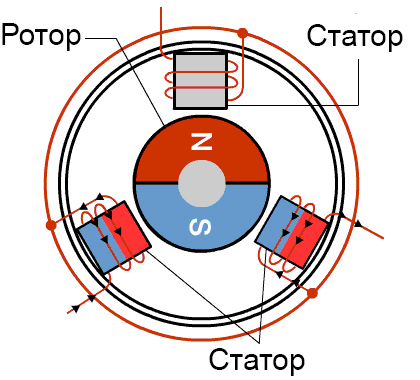
\includegraphics[width=0.5\linewidth]{bldc} 
	\caption{Принципиальная электро-механическая схема моментного трехфазного двигателя \cite[]{BLDC}}
	\label{fig:BLDC}
\end{figure}

В качестве датчиков положения ротора в БДПТ применяются датчики Холла, а в ВД — вращающиеся трансформаторы и накапливающие датчики. В т. н. «бездатчиковых» системах информация о положении определяется системой управления по мгновенным значениям фазных токов.

Информация о положении ротора обрабатывается микропроцессором, который, согласно программе управления, вырабатывает управляющие ШИМ-сигналы. Низковольтные ШИМ-сигналы микроконтроллера затем преобразуются усилителем мощности (обычно транзисторным мостом) в силовые напряжения, подаваемые на двигатель.

Совокупность датчика положения ротора и электронного узла в ВД и БДПТ можно с определённой долей достоверности сравнить с щёточно-коллекторным узлом ДПТ. Однако следует помнить, что двигатели редко применяются вне электропривода. Таким образом, электронная аппаратура характерна для ВД почти в той же степени, что и для ДПТ. \cite[]{BLDC}



\subsection{Электрическая модель} \label{sec:ch3/sec9/sub4}
Трехфазный ДБМ собраный по схеме звезда может быть описан тремя уравнениями \cite[]{BLDC_Stefan}:

\begin{equation}
\label{eq:p3:9.1}
\begin{alignedat}{2}
u_{ab} = R (i_a - i_b) + L \dfrac{d}{dt} (i_a - i_b) + e_a - e_b \\
u_{bc} = R (i_b - i_c) + L \dfrac{d}{dt} (i_b - i_c) + e_b - e_c \\
u_{ca} = R (i_c - i_a) + L \dfrac{d}{dt} (i_c - i_a) + e_c - e_a
\end{alignedat}
\end{equation}
где 
$U$ - межфазнеое напряжение, 
$e$ - обратнонаведенное ЭДС, 
$i$ - фазовый ток, 
$R$ - сопротивление фазы постоянному току, 
$L$ - индуктивность приведенная к фазе.

Обратнонаведенное ЭДС описывается следующим уравнением:
\begin{equation}
\label{eq:p3:9.2}
\begin{alignedat}{2}
\overline{e} = (e_a, e_b, e_c) = C_e \dot{\alpha}_m \overline{F}(\frac{\textit{P}}{2}\alpha_m)\\
\end{alignedat}
\end{equation}
где 
$\overline{e}$ - вектор обратнонаведенных эдс, 
$C_e$ - приведенный к фазе коэффициент ЭДС $[\frac{\textit{В с}}{\textit{рад}} ]$,
$\alpha_m$ - положение вращения ротора, 
$\dot{\alpha}_m$ - угловая скорость вращения ротора, 
$\textit{P}$ - количество пар полюсов электродвигателя, 
вектор-функция распределения магнитного между фазами описывается следующим образом \cite[]{MATLAB1}:

\begin{equation}
\label{eq:p3:9.3}
\begin{alignedat}{2}
\overline{F}(\alpha) = \left( \begin{matrix}
\cos (\alpha) \\
\cos (\alpha - \frac{2 \pi}{3}) \\
\cos (\alpha + \frac{2 \pi}{3}) \\
\end{matrix}
\right) \\
\end{alignedat}
\end{equation}

Электрический крутящий момент запишется в следующем виде:
\begin{equation}
\label{eq:p3:9.4}
\begin{alignedat}{2}
M_{\textit{дв.x}} = C_m <\overline{F}(\frac{\textit{P}}{2}\alpha_m),\overline{i}>
\end{alignedat}
\end{equation}
где
$C_m$ - приведенный к фазе коэффициент момента $[\frac{\textit{Н м}}{\textit{А}} ]$,
$\overline{i} = (i_a, i_b, i_c)$ - вектор фазовых токов.

\subsection{Линеаризованные уравнения привода} \label{sec:ch3/sec9/linearize}

Линеаризованное уравнение привода запишется в следующем виде:
\begin{equation}
\label{eq:p3:lin1}
\begin{alignedat}{2}
\left.
\begin{matrix}
M_{\textit{дв.x}} = C_m i\\
U = R i + L \dfrac{d i}{dt} + C_e \dot{\alpha}_m \\
\end{matrix}
\right\rbrace 
\end{alignedat}
\end{equation}

Уравнение (\labelcref{eq:p3:lin1}), представив в операторной форме, преобразуем и выразим относительно координаты управления:

\begin{equation}
\label{eq:p3:lin2}
\begin{multlined}
\left.
\begin{matrix}
M_{\textit{дв.x}} = C_m i\\
U = R i + L p i + C_e p \alpha_m \\
\end{matrix}
\right\rbrace \\
\alpha_m = \frac{1}{C_e p} U - \frac{R + L p}{C_m C_e p} M_{\textit{дв.x}},\\
\alpha_m = W_n(p) U - W_f(p) M_{\textit{дв.x}},
\end{multlined}
\end{equation}
где
$W_n(p) = \frac{1}{C_e p}$ - передаточная функция (ПФ) по управлению,

$W_f(p) = \frac{R + L p}{C_m C_e p}$ - передаточная функция по возмущению от моментов нагрузки.

Или относительно момента силы:

\begin{equation}
\label{eq:p3:lin2+}
\begin{multlined}
M_{\textit{дв.x}} = \frac{C_m}{R + L p} U - \frac{C_m C_e}{R + L p} \dot\alpha_m,\\
M_{\textit{дв.x}} = k U - b \dot\alpha_m,
\end{multlined}
\end{equation}
где
$k = \frac{C_m}{R + L p}$,
$b = \frac{C_m C_e}{R + L p}$.

Обозначим уравнения описывающие привод для каждого из каналов в соответствии:

\begin{equation}
\label{eq:p3:lin3}
\begin{multlined}
\alpha_{m.x} = W_{n.x}(p) U_x - W_{f.x}(p) M_{\textit{дв.x}},
\end{multlined}
\end{equation}
где 
$W_{n.x}(p) = \frac{1}{C_{e.x} p}$,

$W_{f.x}(p) = \frac{R_x + L_x p}{C_{m.x} C_{e.x} p}$,

$x = (1,2)$ - номер соответствующего канала управления.

Или относительно момента силы:

\begin{equation}
\label{eq:p3:lin4}
\begin{multlined}
M_{\textit{дв.x}} = k_x U_x - b_x \dot\alpha_{m.x},
\end{multlined}
\end{equation}
где
$k_x = \frac{C_{m.x}}{R_x + L_x p}$,
$b_x = \frac{C_{m.x} C_{e.x}}{R_x + L_x p}$.

\begin{comment}
\subsection{Механическая модель} \label{sec:ch3/sec9/sub3}

\todo{привести в соответствие с 3.3.2}

\todo{литература}

С точки зрения механики электродивгатель рассматривается как система с одной степенью свободы. Запишем уравнение (\labelcref{eq:p3:48}) относительно привода:

\begin{equation}
\label{eq:p3:9.5}
\begin{alignedat}{2}
M_e - M_{\textit{L}} - M_{\textit{тр}} = J \ddot{\alpha}_m 
\end{alignedat}
\end{equation}
где 
$M_{\textit{L}} = M_{\textit{дб}} + M_{\textit{н}}$ - крутящий момент нагрузки, складывается из момента дисбаланса ($M_{\textit{дб}}$) и момента обусловленного движением носителя ($M_{\textit{н}}$), 
$M_{\textit{тр}}$ - момент трения, 
$J = J_{p} + J_{H}$ - суммарный момент инерции, складывается из момента инерции ротора ($J_{p}$) и нагрузки ($J_{H}$), 
$\ddot{\alpha}_m $ - угловое ускорение вращения ротора.

Момент силы трения определяется по формуле: 
\begin{equation}
\label{eq:p3:9.6}
\begin{alignedat}{2}
M_{\textit{тр}} = M_{\textit{тр}}^{\textit{max}} sign( \dot{\alpha}_m ),
\end{alignedat}
\end{equation}
где
$M_{\textit{тр}}^{\textit{max}} = (2..5) 10^{-3} m$ - максимальный момент трения [26],
$m$ - масса подвижной части.

Момент силы дисбаланса нагрузки определим по формуле:
\begin{equation}
\label{eq:p3:9.7}
\begin{alignedat}{2}
\vec{M}_{\textit{дб}} = 
m\left[{\vec {r_0}}\times {(\vec {a} + \vec {g})}\right],} 
\end{alignedat}
\end{equation}
где
$\vec{a}$ - ускорение носителя,
$\vec{g}$ - ускорение свободного падения,
$\vec {r_0} = ( x^2_0, y^2_0) $ - положение центра масс относительно оси вращения.

Момент силы обусловленный движением носителя:
\begin{equation}
\label{eq:p3:9.8}
\begin{alignedat}{2}
M_{\textit{н}} = J \ddot{\alpha_{\textit{ла}}}
\end{alignedat}
\end{equation}
где 
$\ddot{\alpha_{\textit{ла}}}$ - угловое ускорение носителя
\end{comment}

\section{Методика линеаризации} \label{ch:ch3/linerization}

\cite[]{tailor}

Для получения формулы Тейлора функции n переменных $f(x) = f(x_1, x_2, ... x_n)$, которая в некоторой окрестности точки  
$ x_0 = (a_{1},a_{2},...,a_{n})$ имеет непрерывные производные до  $(m+1)$ - го порядка включительно, введём дифференциальный оператор

$ \mathrm {T} =(x_{1}-a_{1}){\dfrac {\partial }{\partial x_{1}}}+(x_{2}-a_{2}){\dfrac {\partial }{\partial x_{2}}}+...+(x_{n}-a_{n}){\dfrac {\partial }{\partial x_{n}}}.$ 
Тогда разложение (формула Тейлора) функции по степеням  $ (x_{i}-a_{i})^{k_{i}}$ в окрестности точки   $(a_{1},a_{2},...,a_{n})$ имеет вид

 $ f(x_{1},x_{2},...x_{n})=\sum \limits _{k=0}^{m}{\dfrac {\mathrm {T} ^{k}f(a_{1},a_{2},...,a_{n})}{k!}}+R_{m}(x_{1},x_{2},...x_{n}),$
 
где $ R_m(x_1, x_2, ... x_n)$ — остаточный член порядка $(m+1)$.

При линеаризации нелинейных уравнений предполагаем, что в динамическом процессе отклонения переменных относительно невозмущенного движения остаются все время малыми:

$x_i = {x_0}_i + \Delta x_i$

Разложив функцию в ряд по степеням малых отклонений () переменных и оставив только члены ряда первого порядка малости, получим линейное дифференциальное уравнение в отклонениях:

$ f(x) = f(x_0) + T f(x_0) (\Delta x)$

\section{Линеаризованная система} \label{ch:ch3/sect10}

Ввиду сложности исследований нелинейных дифференциальных уравнений пространственного движения ОЭП, как объекта управления (ОУ), рассмотрим частный случай этих уравнений, когда объект управления установлен на неподвижном основании или на ЛА, совершающем поступательное равномерное прямолинейное движение в горизонтальной плоскости ( \( \psi =0, \vartheta =0, \gamma =0 \) ), установочные углы: \( \psi _{y}=0, \vartheta _{y}=0, \gamma _{y}=0 \) \ и вибрации не учитываются. В уравнение (\labelcref{eq:p3:49}) подставим (\labelcref{eq:p3:lin4}):

\begin{equation}%\tag{3.50}
\label{eq:p3:50}
\begin{multlined}
\left( B_{1}+B \left( \beta \right) \right) \ddot \alpha -D \left( \beta \right) \ddot \beta -2F \left( \beta \right) \dot \alpha \dot \beta -E \left( \beta \right) \dot \beta ^{2}=\\
k_{1}u_{1}-b_{1} \dot \alpha -M_{\textit{тр.1}}sign \left( \dot \alpha \right) 
\end{multlined}
\end{equation}

\begin{equation}%\tag{3.51}
\label{eq:p3:51}
\begin{multlined}
C_{2} \ddot \beta -D \left( \beta \right) \ddot \alpha +F \left( \beta \right) \dot \alpha ^{2}=\\
-m_{2}g \left( 
x_{C_{2}}cos \left( \beta \right) -
y_{C_{2}}sin \left( \beta \right) 
\right) 
+k_{2}u_{2}-
b_{2} \dot \beta _{2}-M_{\textit{тр.2}}sign \left( \dot \beta \right) 
\end{multlined}
\end{equation}
Здесь и далее будем придерживаться обозначений, принятых в разделе \ref{sec:ch3/sec8}. 

\begin{equation}%\tag{3.52}
\label{eq:p3:52}
\begin{multlined}
B \left( \beta \right) =\frac{A_{2}+B_{2}}{2}-\frac{A_{2}-B_{2}}{2}cos \left( 2 \beta \right) -F_{2}sin \left( 2 \beta \right),\\
F \left( \beta \right) =F_{2}cos \left( 2 \beta \right) -\frac{A_{2}-B_{2}}{2}sin \left( 2 \beta \right),\\
E \left( \beta \right) =E_{2}cos \left( \beta \right) -D_{2}sin \left( \beta \right),\\
D \left( \beta \right) =D_{2}cos \left( \beta \right) +E_{2}sin \left( \beta \right), \\
A_{2} \left( \beta \right) =\frac{A_{2}-B_{2}}{2}cos \left( 2 \beta \right) +F_{2}sin \left( 2 \beta \right),
\end{multlined}
\end{equation}
Принятые уравнения (\labelcref{eq:p3:50}),(\labelcref{eq:p3:51}) все же являются нелинейными с нелинейными перекрестными связями. Для оценки динамических свойств ОУ проведем линеаризацию нелинейностей уравнений (\labelcref{eq:p3:50}),(\labelcref{eq:p3:51}) относительно установившегося процесса движения ОУ (примем его за невозмущенное движение), имеющего место при некоторых постоянных значениях: 
\begin{equation}%\tag{3.53}
\label{eq:p3:53}
\begin{multlined}
\alpha _{0}, \ \beta _{0}, \ \dot \alpha _{0}=\dot \beta _{0}=\ddot \alpha _{0}=\ddot \beta _{0}=0, \ u_{10}, \ u_{20}, \ M_{\textit{тр10}}, \ M_{\textit{тр20}}.
\end{multlined}
\end{equation}
При линеаризации нелинейных уравнений предполагаем, что в динамическом процессе отклонения переменных относительно невозмущенного движения остаются все время малыми: 
\begin{equation}%\tag{3.54}
\label{eq:p3:54}
\begin{multlined}
\alpha = \alpha _{0}+ \Delta \alpha, \ 
\beta = \beta _{0}+ \Delta \beta, \ 
\dot \alpha = \Delta \dot \alpha, \ 
\dot \beta = \Delta \dot \beta, \ 
\ddot \alpha = \Delta \ddot \alpha, \ 
\ddot \beta = \Delta \ddot \beta,\\
u_{1}=u_{10}+ \Delta u_{1}, \ 
u_{2}=u_{20}+ \Delta u_{2}, \ 
M_{\textit{тр1}}=M_{\textit{тр10}}+ \Delta М_{1}, \ 
M_{\textit{тр2}}=M_{тр20}+ \Delta М_{2}.
\end{multlined}
\end{equation}
Разложив нелинейные функции уравнений (\labelcref{eq:p3:50}),(\labelcref{eq:p3:51}) в ряд по степеням малых отклонений переменных и оставив только члены ряда первого порядка малости, получим линейные дифференциальные уравнения в отклонениях: 

\begin{equation}
\label{eq:p3:55}
\begin{multlined}
\left( B_{1}+B \left( \beta _{0} \right) \right) \Delta \ddot \alpha -
2F \left( \beta _{0} \right)\dot \alpha _{0} \Delta \beta -
D \left( \beta _{0} \right) \Delta \ddot \beta +
E \left( \beta _{0} \right) \ddot \beta _{0} \Delta \beta -\\
2F \left( \beta _{0} \right) \dot \alpha _{0} \Delta \dot \beta -
2F \left( \beta _{0} \right) \dot \beta _{0} \Delta \dot \alpha -\\
2A_{2} \left( \beta _{0} \right) \dot \beta _{0} \dot \alpha _{0} \Delta \beta -
2E \left( \beta _{0} \right) \dot \beta _{0} \Delta \dot \beta -
D \left( \beta _{0} \right) \dot \beta _{0}^{2} \Delta \beta \\
\dot \omega _{y_{y}} ( t ) ( B_{1}+B ( \beta_0 ) )=\\
k_{1} \Delta u-
b_{1} \Delta \dot \alpha - \Delta M_{1}sign \left( \Delta \dot \alpha \right)
\end{multlined}
\end{equation}
\begin{equation}
\label{eq:p3:56}
\begin{multlined}
C_{2} \Delta \ddot \beta -
D \left( \beta _{0} \right) \Delta \ddot \alpha +
E \left( \beta _{0} \right) \ddot \alpha _{0} \Delta \beta +
2F \left( \beta _{0} \right) \dot \alpha _{0} \Delta \dot \alpha +
2A_{2} \left( \beta _{0} \right) \dot \alpha _{0}^{2} \Delta \beta \\
\dot \omega _{z_{y}} \left( t \right) \left[ E \left( \beta_0 \right) sin \left( \alpha_0 \right) +C_{2}cos \left( \alpha_0 \right) \right]-\\
m_{2}g \left( 
x_{C_{2}}sin \left( \beta _{0} \right) -
y_{C_{2}}cos \left( \beta _{0} \right) 
\right) =
k_{2} \Delta u_{2}-
b_{2} \Delta \dot \beta - 
\Delta M_{2}sign \left( \Delta \dot \beta \right) 
\end{multlined}
\end{equation}
где \( \alpha _{0}, \beta _{0} \) \ могут принимать любые значения в области, заданных ТЗ. 

С учетом (\labelcref{eq:p3:53}) уравнения (\labelcref{eq:p3:55}),(\labelcref{eq:p3:56}) упростятся: 
\begin{equation}
\label{eq:p3:57}
\begin{multlined}
\left( B_{1}+B \left( \beta _{0} \right) \right) \Delta \ddot \alpha -
D \left( \beta _{0} \right) \Delta \ddot \beta +\\
\dot \omega _{y_{y}} ( t ) ( B_{1}+B ( \beta_0 ) )
=
k_{1} \Delta u_{1} -
b_{1} \Delta \dot \alpha - 
\Delta M_{1}sign \left( \Delta \dot \alpha \right) 
\end{multlined}
\end{equation}
\begin{equation}
\label{eq:p3:58}
\begin{multlined}
C_{2} \Delta \ddot \beta -
D \left( \beta _{0} \right) \Delta \ddot \alpha +
\dot \omega _{z_{y}} \left( t \right) \left[ E \left( \beta_0 \right) sin \left( \alpha_0 \right) +C_{2}cos \left( \alpha_0 \right) \right]-\\
m_{2}g \left( x_{C_{2}}sin \left( \beta _{0} \right) -
y_{C_{2}}cos \left( \beta _{0} \right) \right) 
=\\
k_{2} \Delta u_{2}-
b_{2} \Delta \dot \beta - 
\Delta M_{2}sign \left( \Delta \dot \beta \right) 
\end{multlined}
\end{equation}
Учитывая $\dot \omega _{y_{y}} ( t ) = \ddot \psi, \dot \omega _{z_{y}} ( t ) = \ddot \vartheta$, перепишем уравнения (\labelcref{eq:p3:57}),(\labelcref{eq:p3:58}) в операторной форме: 


%\tag{3.59}
\begin{equation}
\label{eq:p3:59}
\begin{multlined}
\left( a_{11}p^{2}+b_{11}p \right) \Delta \alpha -
a_{12}p^{2} \Delta \beta + 
a_{11} p^2 \Delta \psi 
=\\
k_{1} \Delta u_{1}- 
\Delta M_{1}sign \left( p \Delta \alpha \right),\\
-a_{21}p^{2} \Delta \alpha + 
\left( a_{22}p^{2}+b_{22}p \right) \Delta \beta +c_{22}+
 d_{23} p^2 \Delta \vartheta
=\\
k_{2} \Delta u_{2}- \Delta M_{2}sign \left( p \Delta \beta \right),
\end{multlined}
\end{equation}

где 
\( a_{11}=B_{1}+B \left( \beta _{0} \right), 
\ a_{12}=D \left( \beta _{0} \right), 
\ b_{11}=b_{1}, 
\) \[ a_{22}=C_{2}, 
\ a_{21}=D \left( \beta _{0} \right), 
\ c_{22}=-m_{2}g \left( x_{C_{2}}sin \left( \beta _{0} \right) -y_{C_{2}}cos \left( \beta _{0} \right) \right), \
 b_{22}=b_{2}, \] 

$d_{23} = \left[ E \left( \beta_0 \right) sin \left( \alpha_0 \right) +C_{2}cos \left( \alpha_0 \right) \right]$.

Из уравнений (\labelcref{eq:p3:59}) видно, что существуют перекрестные связи пропорциональные центробежным моментам инерции ОЭП по углу места. Далее для синтеза регуляторов изолированных каналов управления воспользуемся результатами работы [], где проведена в частотной области оценка влияния динамических перекрестных связей на устойчивость и качество регулирования ОЭП, и показано, что перекрестные связи между каналами управления влияют друг на друга незначительно. В связи с этим синтез регуляторов по азимуту и углу места можно проводить независимо друг от друга. 


\section{Выводы по главе} \label{ch:ch3/sect11}

Разработаная математическая модель описывает ОЭП с точки зрения законов динамики и уравнений описывающих электрические машины. На основании этих законов было сделано следующее:
\begin{enumerate}
	\item Описана механическая модель БОЭП,
	\item Получены уравнения динамики системы с учетом движения носителя и перекрестных связей,
	\item Описана механическая и электрическая модель привода,
	\item Приведены линеаризованные уравнения привода,
	\item Произведена линеаризация системы,
	\item Получены уравнения пригодные для разработки алгоритмов управления БОЭП.
\end{enumerate}
Используя эти уравнения с применением компьютерных технологий можно решать задачи синтеза САУ и СВ бортовых ОЭП.

\clearpage